\documentclass[a4paper, 11pt, twoside]{report}
% Remember to follow the rules for AAU report format
% - Spacing must be minimum 1.2
% - Font size must be minimum 11
% - Margins must be at least 2 cm., including 3 cm. in the binding margin
% Others:
\usepackage{titlesec}
%%%%%% Headers
\usepackage{fancyhdr}
\usepackage[paper=a4paper,layout=a4paper]{geometry}
\usepackage[pages=some]{background}
\usepackage{tikz}
\usetikzlibrary{positioning, shapes, arrows, fit, automata}
\usepackage{amsmath}  
\usepackage{amssymb}  
\usepackage{calc}  
\usepackage[utf8]{inputenc}
\usepackage[english]{babel}
\usepackage{blindtext}
\usepackage{bm,times}
\newcommand{\mx}[1]{\mathbf{\bm{#1}}} % Matrix command
\newcommand{\vc}[1]{\mathbf{\bm{#1}}} % Vector command
\usepackage{hyperref, bookmark, url}
\usepackage{graphicx}
\usepackage{float} 
\usepackage{lastpage} 
\usepackage{listings}
\usepackage{xcolor,colortbl}
\bibliographystyle{ieeetr}
\usepackage[nottoc]{tocbibind} % to add the bibliography to the table of contents, add the option numbib for adding a chapter number to it
% To prevent Latex moving the tables around:
\usepackage{float}
\restylefloat{table}
%%%%%%% Commands  
\titleformat{\chapter}{\normalfont\huge\bfseries}{\thechapter}{1em}{}

\setlength{\columnsep}{1cm}
\setlength{\headheight}{13.6pt}

\definecolor{aaublue}{RGB}{33,26,82}
\definecolor{link}{RGB}{6, 69, 173}
\definecolor{maroon}{cmyk}{0, 0.73, 1, 0.30}
\definecolor{halfgray}{gray}{0.55}

\definecolor{navyblue}{RGB}{22, 22, 110}
\definecolor{bloo}{RGB}{15, 30, 127}
\definecolor{Groon}{RGB}{72,188,60}
\definecolor{pink}{rgb}{0.858, 0.188, 0.478}

\usepackage[font={color=navyblue,small},figurename=Fig.,labelfont={it}]{caption}

\definecolor{aaublue}{RGB}{33,26,82}
\definecolor{link}{RGB}{6, 69, 173}
\definecolor{maroon}{cmyk}{0, 0.73, 1, 0.30}
\definecolor{halfgray}{gray}{0.55}

  
%%% Style for C code
\definecolor{mGreen}{rgb}{0,0.6,0}
\definecolor{mGray}{rgb}{0.5,0.5,0.5}
\definecolor{mPurple}{rgb}{0.58,0,0.82}
\definecolor{backgroundColour}{rgb}{0.95,0.95,0.92}

\lstdefinestyle{CStyle}{
    backgroundcolor=\color{backgroundColour},   
    commentstyle=\color{mGreen},
    keywordstyle=\color{magenta},
    numberstyle=\tiny\color{mGray},
    stringstyle=\color{mPurple},
    basicstyle=\ttfamily\footnotesize,
    breakatwhitespace=false,         
    breaklines=true,                 
    captionpos=b,                    
    keepspaces=true,                 
    numbers=left,                    
    numbersep=5pt,                  
    showspaces=false,                
    showstringspaces=false,
    showtabs=false,                  
    tabsize=2,
    language=C
}
%%% Style for Basch commands
\lstdefinestyle{BStyle}{
    backgroundcolor=\color{backgroundColour},   
    commentstyle=\color{brown},
    keywordstyle=\color{blue},
    numberstyle=\tiny\color{mGray},
    stringstyle=\color{violet},
    basicstyle=\ttfamily\footnotesize,
    breakatwhitespace=false,         
    breaklines=true,                 
    captionpos=b,                    
    keepspaces=true,                 
    numbers=left,                    
    numbersep=5pt,                  
    showspaces=false,                
    showstringspaces=false,
    showtabs=false,                  
    tabsize=2,
    language=bash
}

%%% Style other languages
\lstdefinestyle{OtherSt}{
    backgroundcolor=\color{backgroundColour},   
    commentstyle=\color{darkgray},
    keywordstyle=\color{brown},
    numberstyle=\tiny\color{mGray},
    stringstyle=\color{olive},
    basicstyle=\ttfamily\footnotesize,
    breakatwhitespace=false,         
    breaklines=true,                 
    captionpos=b,                    
    keepspaces=true,                 
    numbers=left,                    
    numbersep=5pt,                  
    showspaces=false,                
    showstringspaces=false,
    showtabs=false,                  
    tabsize=2,
}
% Basic colors avaliable in the xcolor package: black, blue, brown, cyan, darkgray, gray, green, lightgray, lime, magenta, olive, orange, pink, purple, red, teal, violet, white, yellow.

\begin{document}

% ================================ Front pages ===========================
\pagenumbering{roman}
\backgroundsetup{
scale=1.1,
angle=0,
opacity=1.0,  %% adjust
contents={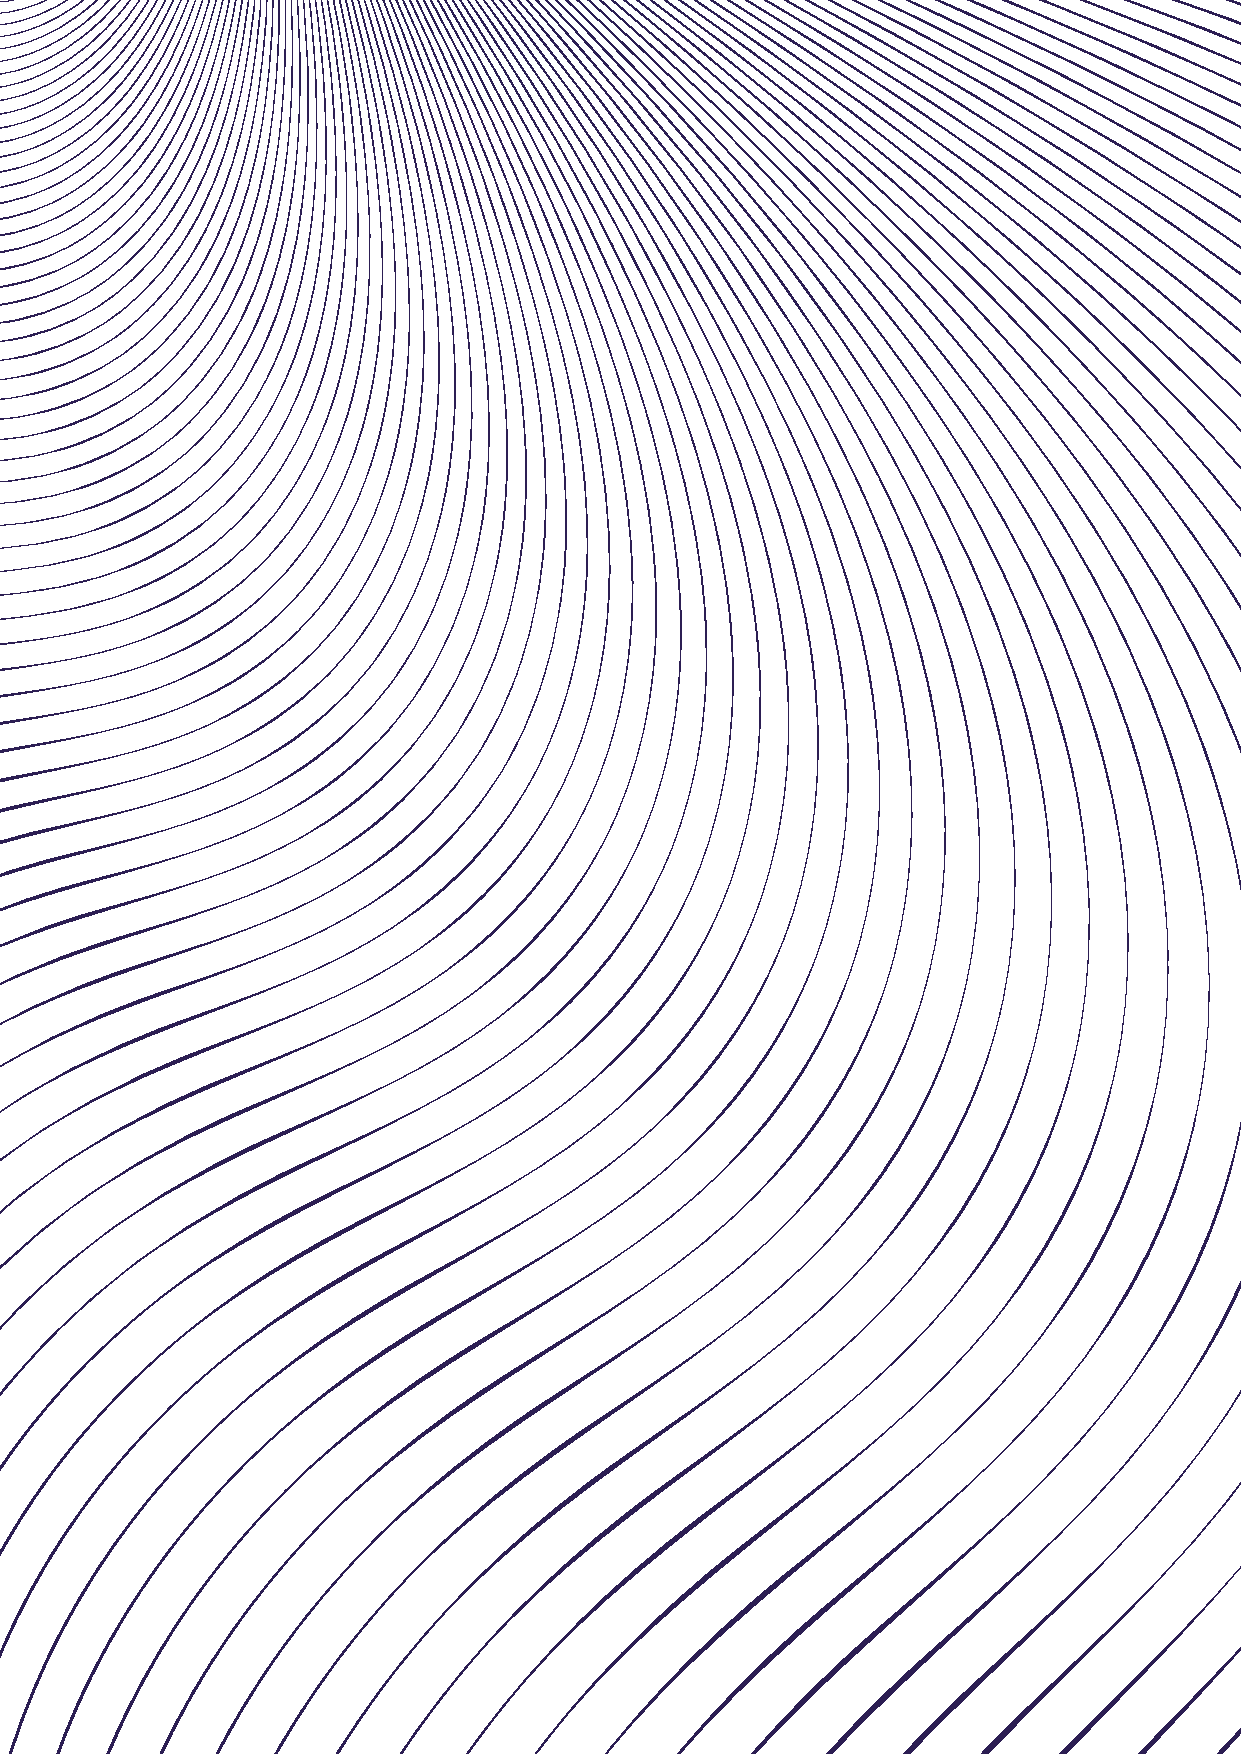
\includegraphics[width=\paperwidth,height=\paperheight]{Figures/frontpage/aau_waves}}
}
% The geometry for this page is different and it is only applied in this section:
\begin{titlepage}

\newgeometry{top=0cm,bottom=1.2cm,right=0cm,left=0cm}
\BgThispage

%Top image
% For the ubuntu logo:
%  \centerline{
\includegraphics[totalheight=0.568\paperwidth,width=1\paperwidth]{Figures/frontpage/frontpageimage1.jpg}}%
  \begin{center} 
  \centerline{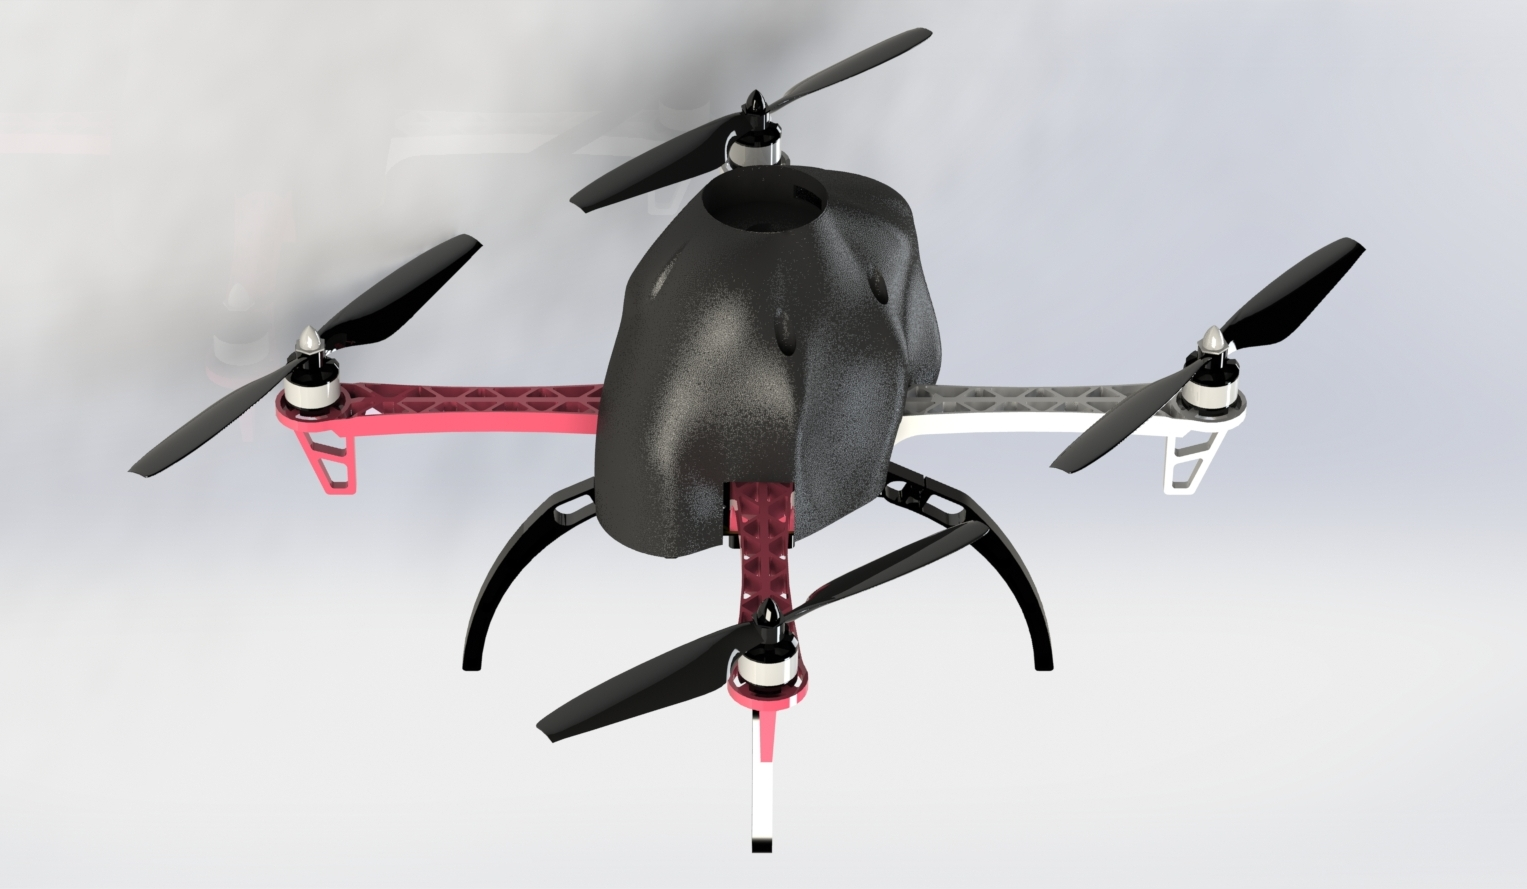
\includegraphics[totalheight=0.5822\paperwidth,width=1\paperwidth]{Figures/frontpage/render_frontpage.jpg}}% 
  \end{center}

%Title stuff	
	\vspace*{-0.96cm}
  {\noindent\color{aaublue}\fboxsep0pt\colorbox{white}{\begin{tabular}{@{}p{\paperwidth}@{}}
    \centerline{
    \begin{minipage}{0.85\textwidth}
        \bigskip
				\bigskip
        \centering
        \Huge{\textbf{PREDICT Project documentation}}
    \end{minipage}}
		
	\centerline{
	\begin{minipage}{0.9\textwidth}
        \bigskip
        \centering
        \Large{Working of a flight controller in a multi-core PATMOS architecture}
    \end{minipage}}
			
	\centerline{
	\begin{minipage}{0.9\textwidth}
        \bigskip
        \centering
        {\Large Carolina Gomez Salvatierra, Mark Adamik, Rahul Ravichandran}
    \end{minipage}}
			
    \centerline{
    \begin{minipage}{0.9\textwidth}
        \bigskip
        \centering
        {\large Department of Electronic Systems} 
    \end{minipage}}
			
    \centerline{
    \begin{minipage}{0.9\textwidth}
        \bigskip
        \centering
        {\Large 15th April, 2021}
        \smallskip
    \end{minipage}}
			
  \end{tabular}}}
  \vfill
  \begin{figure}[!b]
	\centering
    
\includegraphics[width=0.2\paperwidth]{Figures/frontpage/AAUcircle.png}
  \end{figure}

\end{titlepage}
\clearpage

\restoregeometry %Remember to set geometry defaults back after the page
\hypersetup{pageanchor=false} % To avoid problems with hyperref package
\thispagestyle{empty}
{\small
\strut\vfill
\noindent \copyright{} Department of Electronic Systems, Aalborg University, 2020-21.\par
\vspace{0.3cm}
\subsubsection*{Attributions}
This document was typeset using \LaTeX \hspace{0.05cm} and Quartus Prime for the Real-Time system architecture.
\noindent
%---> Here you can write something about which tools and software you have used for typesetting the document, running simulations and creating figures. If you do not know what to write, either leave this page blank or have a look at the colophon in some of your books.\par
%\vspace{0.2cm}
}
\clearpage
\hypersetup{pageanchor=true} % Reenable this.

\titleformat{\chapter}{\normalfont\huge\bfseries}{\thechapter}{1em}{}

\newpage
%The formatting for the title 'paragraph'

\section*{Acknowledgment}
The project was completed due to support from project supervisor Anders la Cour-Harbo and also due to the cooperation with DTU team members.
%%% =========================== ORIGINAL ===================================
\newpage
\section*{Abbreviations List}

\begin{figure}[H]
   \begin{center}
       \begin{tabular}{ ll }
            \textbf{Abbreviation}   &       \textbf{Definition}  
            \\
            AAU                     &       Aalborg University 
            \\
            AMR                     &       Autonomous Mobile Robot    
             \\
            CoM                     &       Center of Mass
            \\
            DOF                     &       Degree of Freedom
            \\
            DTU                     &       Technical University of Denmark
            \\
            FPGA                    &       Field Programmable Gate Array
            \\
            GPIO                    &       General Purpose Input/Output
            \\
            GPS                     &       Global Positioning System 
            \\
            I2C                     &       Inter-Integrated Circuit
            \\
            PCB                    &       Printed Circuit Board
            \\
            PWM                     &       Pulse Width Modulation
            \\
            SPI                     &       Serial Peripheral Interface
            \\
            UART                    &       Universal asynchronous receiver-transmitter
            \\
            URDF                    &       Universal Robot Description Format
            \\
            VLIW                    &       Very Long Instruction word
            \\
            VM                      &       Virtual Machine 
        \end{tabular}
   \end{center}
\end{figure}


% ================================ Tables and listing ===========================
\tableofcontents
\listoffigures
\listoftables

% ================================ Document content ===========================
\newpage
\pagenumbering{arabic}
% Redefine the plain page style
\fancypagestyle{plain}{
  \fancyhf{}
  \fancyhead[LE,RO]{\textcolor{halfgray}{Aalborg University}}
  \fancyhead[RE,LO]{\textcolor{halfgray}{PREDICT Project}}
  \fancyfoot[CE,CO]{\textcolor{halfgray}{\thepage}} %\leftmark
  %\fancyfoot[LE,RO]{\textcolor{halfgray}{\chaptername - \thechapter}}
  \renewcommand{\headrulewidth}{0.1pt}
  \renewcommand{\footrulewidth}{0.1pt}
  \renewcommand{\headrule}{\hbox to\headwidth{\color{halfgray}\leaders\hrule height \headrulewidth\hfill}}
  \renewcommand{\footrule}{\hbox to\headwidth{\color{halfgray}\leaders\hrule height \headrulewidth\hfill}}
}
\pagestyle{plain}



\chapter{Introduction}\label{ch:intro}

Patmos is a time-predictable Very Long Instruction word (VLIW) processor developed by Denmark Technical University(DTU). Patmos architecture is a part of the T-Crest Project \cite{bib:t-crest}, whose results were published in  \cite{SCHOEBERL2015449}.  This project describes the construction and development of a quad-copter and its flight controller integrated with the Patmos processor developed by the DTU.

The GitHub repository for the project containing all the test codes and the flight controller code can be found at \cite{bib:multicore_repo}.

\section{Previous works}
% the Arduino guy
This project has been built on top of other researchers and people's work. The most relevant reference is the project YMFC-32 from Joop Brooking\cite{bib:brooking}, the STM32 quad-copter is a DIY low-cost drone with common components that uses an Arduino board for the flight controller development. His work has been very relevant for the flight controller development and electronics design.

% Where we got our additional libraries from
For more specific functionalities, there are also multiple resources for practical Real-Time applications and embedded systems, such as filters, operations or libraries. 
This is the case of the Kalman filter developed by Lauszus\cite{bib:kalmanAAU} and the GPS library by  McGladdery \cite{bib:gpsLib}, whose work has also been used in this project for filtering sensors data and accessing the GPS data.


And in the scenario of using the Patmos architecture, there is Michael Platzer and Emad Jacob Maroun \cite{bib:tu_viena}, who presented a controller for the position of a drone using an IMU. Their work on the I2C communication and corresponding files have been used in this project. 

The fixed point library used in this project is an extension of the code developed by Tim Hartrick and Ivan Voras \cite{bib:fixedpth}.

\section{Problem analysis and project goals}\label{sec:prob_analysis}

The main focus of this project is to develop a drone concept with Patmos that is able to fly, either indoors or outdoors.

The flight controller should also use different features from Patmos and handle them, such as the multi-core for sharing and accessing data between the cores. 

The Patmos libraries has also a variety of functionalities for accessing a data through different communication protocols like Inter-Integrated Circuit (I2C), Serial Peripheral Interface (SPI), 
Universal asynchronous receiver-transmitter (UART) and also send/receive Pulse Width Modulation (PWM), and the board also counts with a set of General Purpose Input/Output (GPIO)  and an analog signals module. 

The Patmos architecture was provided in a Field Programmable Gate Array (FPGA), model De10-Nano and the libraries of Patmos were configured to work with the De10-Nano board. 


Overall, the goals of this project could be listed as follows:

\begin{enumerate}
    \item Design a complete drone, whose design uses different components required for an autonomous flight.
    \item Design a flight controller within Patmos architecture that integrates the different components through the different features provided by Patmos.
    \item The designed drone can take off, fly and land.
    \item The designed drone must be capable of hovering at a constant altitude and and also maintain its position.
    \item The design should be scalable, i.e. it can be easily replicated and reused.
\end{enumerate}

To reach these goals the next chapters in this document shall explain how the problem has been approach. Chapter \ref{ch:hw} presents the hardware design (mechanic and electronics) and Chapter \ref{ch:sw} describes the flight controller design and its features. Then the Chapters \ref{ch:impl} and \ref{ch:test} describes how the design has been implemented and how the libraries of the code provided is structured. Finally, the Chapter \ref{ch:concl} summarizes how the goals have been reached and comments on the project.

Apart from that, there are two additional chapters, Appendixes \ref{app:build} and \ref{app:setup}, which are rather tutorials and more technical explanation about how to mount and assemble the proposed design. These chapters have been written with the idea of being helpful for anybody that wants to replicate this project and/or build on top of it, so this type of reader has instructions and a guideline for doing so.
\chapter{Hardware}\label{ch:hw}

\section{Components}
The aim of this section is to describe in detail the parts and chosen components for this design. Most of these components are quite common among other research projects, and some of them are custom parts.

There are two drone models that were developed for this project, models A and B. 

First, the Table \ref{tab:comp_common} shows the common components for both models. Then, the Table \ref{tab:comp_AB} shows the additional components and to which model they belong to. Finally, the Table \ref{tab:comp_custom} lists the parts that were specifically designed for this project and were done externally.

% mention also adapters and other cablesthat were used during the development?

% Please add the following required packages to your document preamble:
% \usepackage[table,xcdraw]{xcolor}
% If you use beamer only pass "xcolor=table" option, i.e. \documentclass[xcolor=table]{beamer}
\begin{table}[H]

\centering
    \caption{Common components for all models}
    \label{tab:comp_common}
    
\begin{tabular}{lll}
\hline
\rowcolor[HTML]{FFFFFF} 
\multicolumn{1}{|l|}{\cellcolor[HTML]{FFFFFF}Category} & \multicolumn{1}{l|}{\cellcolor[HTML]{FFFFFF}Component} & \multicolumn{1}{l|}{\cellcolor[HTML]{FFFFFF}Description}  \\ \hline
\rowcolor[HTML]{9AFF99} 
Sensors                                                & FTDI LC231X                                            & UART-USB adapter                                                                                                    \\
\rowcolor[HTML]{9AFF99} 
                                                       & FlySky FS-iA6                                          & Receiver                                                                                                             \\
\rowcolor[HTML]{9AFF99} 
                                                       & Turnigy TGY-i6                                                       & Transmitter                                                                                                          \\
\rowcolor[HTML]{9AFF99} 
                                                       & MPU-6050                                               & IMU                                                                                                                  \\
\rowcolor[HTML]{9AFF99} 
                                                       & MS5611                                                 & Barometer                                                                                                            \\
\rowcolor[HTML]{9AFF99} 
                                                       & M8N 8M 8N                                              & GPS and compass                                                                                                      \\
\rowcolor[HTML]{9AFF99} 
                                                       & 3DR Radio 433MHZ                                       & Telemetry                                                                                                            \\
\rowcolor[HTML]{FFFFC7} 
Body                                                   & F450 frame                                             & Frame                                                                                                                \\
\rowcolor[HTML]{FFFFC7} 
                                                       & ZIPPY 2200mAh 3s 40c                                   & Lipo battery                                                                                                         \\
\rowcolor[HTML]{CBCEFB} 
Development                                            & Altera de10-nano                                       & FPGA Board                                                                                                          
\end{tabular}
\end{table}

% Please add the following required packages to your document preamble:
% \usepackage[table,xcdraw]{xcolor}
% If you use beamer only pass "xcolor=table" option, i.e. \documentclass[xcolor=table]{beamer}
\begin{table}[H]

\centering
    \caption{Different components for each model}
    \label{tab:comp_AB}
    
\begin{tabular}{lll}
\hline
\rowcolor[HTML]{FFFFFF} 
\multicolumn{1}{|l|}{\cellcolor[HTML]{FFFFFF}Category} & \multicolumn{1}{l|}{\cellcolor[HTML]{FFFFFF}Component} & \multicolumn{1}{l|}{\cellcolor[HTML]{FFFFFF}Description} \\ \hline
\rowcolor[HTML]{9AFF99} 
Model-A                                                   & Readytosky 2212                                           & Set of 4 motors + ESCs                                                                                                        \\
\rowcolor[HTML]{FFFC9E} 
Model-B                                                   & AirGear 450                                            & Set of 4 motors + ESCs                                                                                                       \\
\rowcolor[HTML]{FFFC9E} 
                                                    & GMP v1.0 XT                                            & Power module                                                                                                        
\end{tabular}
\end{table}

% Please add the following required packages to your document preamble:
% \usepackage[table,xcdraw]{xcolor}
% If you use beamer only pass "xcolor=table" option, i.e. \documentclass[xcolor=table]{beamer}
\begin{table}[H]

\centering
    \caption{Custom components for all models}
    \label{tab:comp_custom}
    
\begin{tabular}{lll}
\hline
\rowcolor[HTML]{FFFFFF} 
\multicolumn{1}{|l|}{\cellcolor[HTML]{FFFFFF}Category} & \multicolumn{1}{l|}{\cellcolor[HTML]{FFFFFF}Desciption} & \multicolumn{1}{l|}{\cellcolor[HTML]{FFFFFF}Designed with} \\ \hline
\rowcolor[HTML]{9AFF99} 
Electronics                                            & PCB                                                     & DipTrace                                                   \\
\rowcolor[HTML]{FFFC9E} 
Mechanics                                                   & Cover                                                   & SolidWorks 2019                                            \\
\rowcolor[HTML]{FFFC9E} 
                                                       & FPGA-Frame attachment                                   & TinkerCAD                                                 \\
\rowcolor[HTML]{FFFC9E} 
                                                       & GPS-Cover attachment                                   & TinkerCAD                                                                                           
\end{tabular}
\end{table}


In case of the model A, most of its components can be bought together as a kit for the Ardupilot F450 Quadcopter \cite{bib:drone_Kit}, which includes the frame, the motors, ESCs, transmitter, receiver, and the GPS-compass.

%% ========================== MECHANICS ==========================
\section{Mechanical design}\label{sec:hw_mec}

\subsection{Assembly}

For both models, the drone type is a quad-copter, with the dimensions of 363mm x 363mm and 152.54mm height. The total weight of the drone with all the components mounted (except the battery) is 1.110kg for the Model-A and 1.170kg for Model-B. Inside the frame, a custom part attaches the FPGA to the top of the frame.

The main mechanical assembly can be seen in Figure \ref{fig:hw_assembA}, which shows the frame, motors, propellers and cover:

\begin{figure} [H]
    \centering
    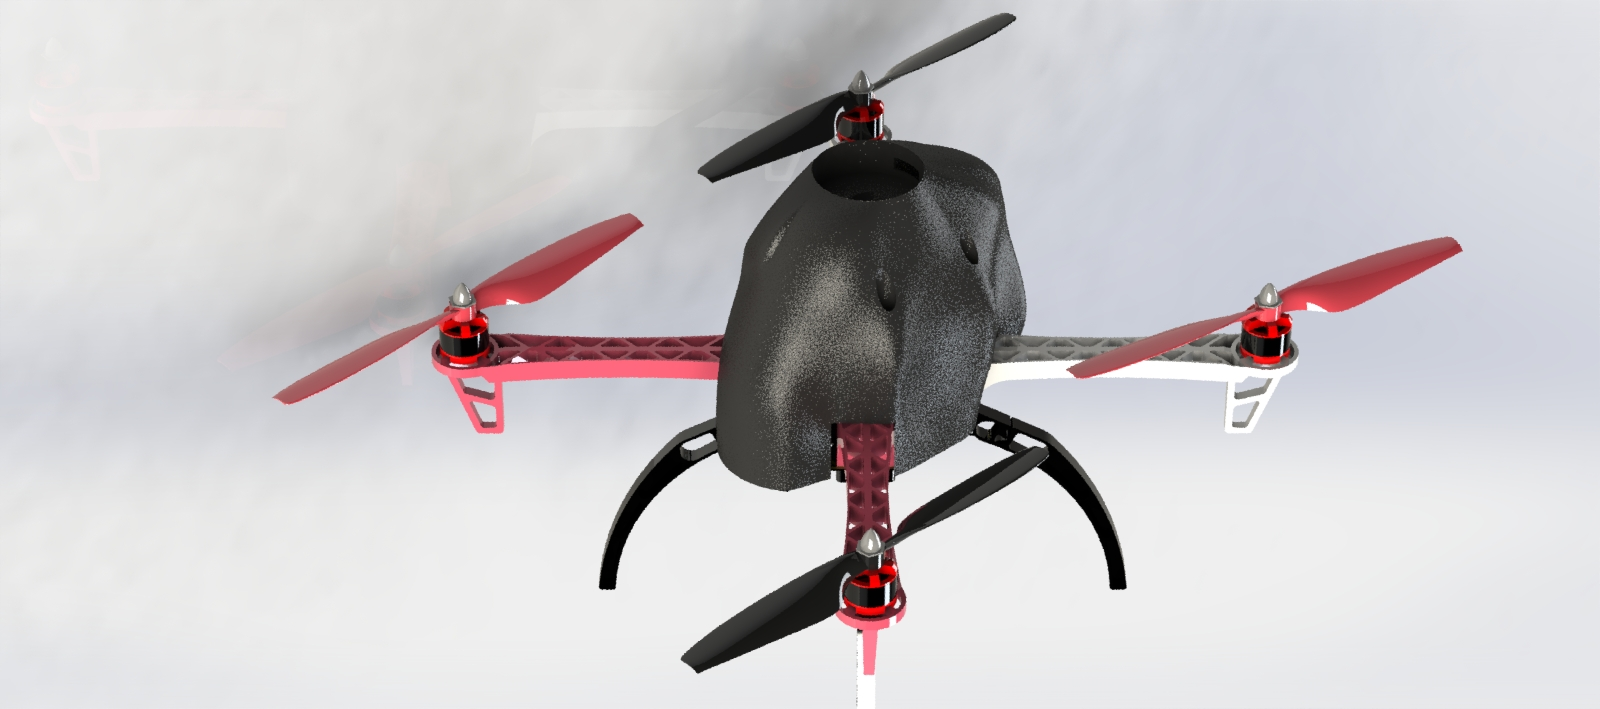
\includegraphics[width=\textwidth]{Figures/hardware/render_assemblyA.JPG}
    \caption{Model A assembly in SolidWorks. Frame, motors and propellers original design from Alejandro Llorente \cite{bib:droneCAD}}
    \label{fig:hw_assembA}
\end{figure}

Inside the frame and cover, the space is distributed as shown in Figure \ref{fig:hw_space}. In case of model B, the only addition to this is that the power module is inside the bottom level, sharing space with the battery: 

\begin{figure} [H]
    \centering
    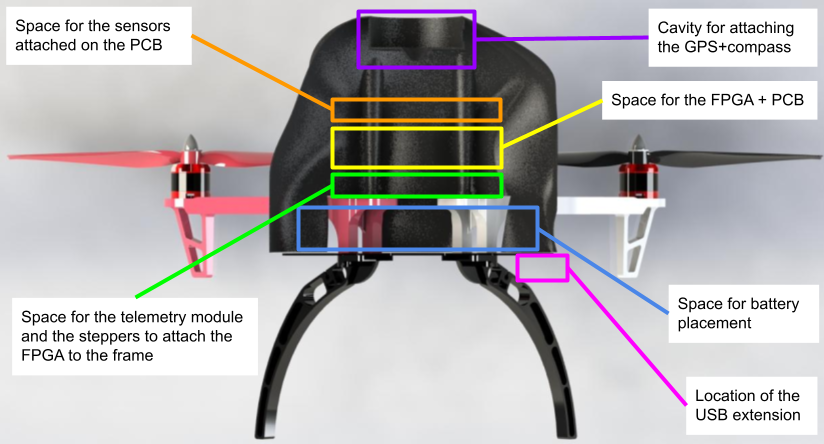
\includegraphics[width=\textwidth]{Figures/hardware/drone_spaces.png}
    \caption{Cut side view of the space distribution for the components inside the Model A assembly. Notice that "Location of the USB extension" refers to a cable extension connected to the UART-USB adapter (located on top of the PCB), so it is possible to download the flight controller application without removing the cover. Also notice that the telemetry module is attached on the same level as the steppers due to its antenna size and therefore it does not fit on top of the PCB as the rest of the sensors.}
    \label{fig:hw_space}
\end{figure}


\subsection{Custom body parts}

As seen on the Table \ref{tab:comp_custom}, some components of the project are custom and therefore, exclusively designed for this project. This subsection describes the mechanical parts, which are the cover, the GPS attachment the FPGA-Frame attachment. All three parts got done with the 3D printers at Aalborg University.

As an overview, the cover and the FPGA-Frame parts are attached to the top of the frame. In case of the GPS attachment, it is a top that holds the GPS on the cover. 


First, the FPGA-Frame attachment is a support part that allows to attach the FPGA to the body, since the drone frame was meant to be used with another controller. This attachment part is shown in Figure \ref{fig:hw_fpgaBase}  and its size is of 70.59mm x 109.54mm and a thickness of 2 mm.

\begin{figure}[!htb]
    \centering
    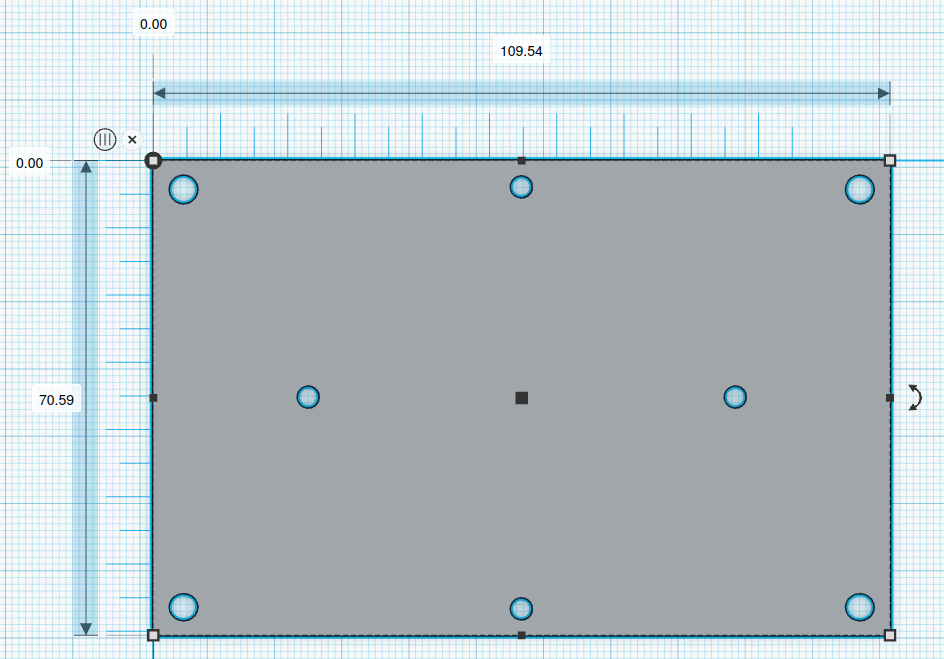
\includegraphics[width=\textwidth]{Figures/hardware/fpga_attachment.png}
    \caption{FPGA-Frame attachment custom part. The four holes on the corners are for the FGPA and the four holes on the center are for the body frame. All screws and steppers are size M3. The length for the steppers is 6mm.}
    \label{fig:hw_fpgaBase}
\end{figure}


Secondly, the cover protects the components and the board from possible impacts and other unexpected events during the fly. The cover is shown in Figure \ref{fig:hw_cover}, which has a size of 194.81mm x 131.46mm, a total height of 158.84mm and a thickness of 0.75mm:

\begin{figure}[!h]
    \centering
    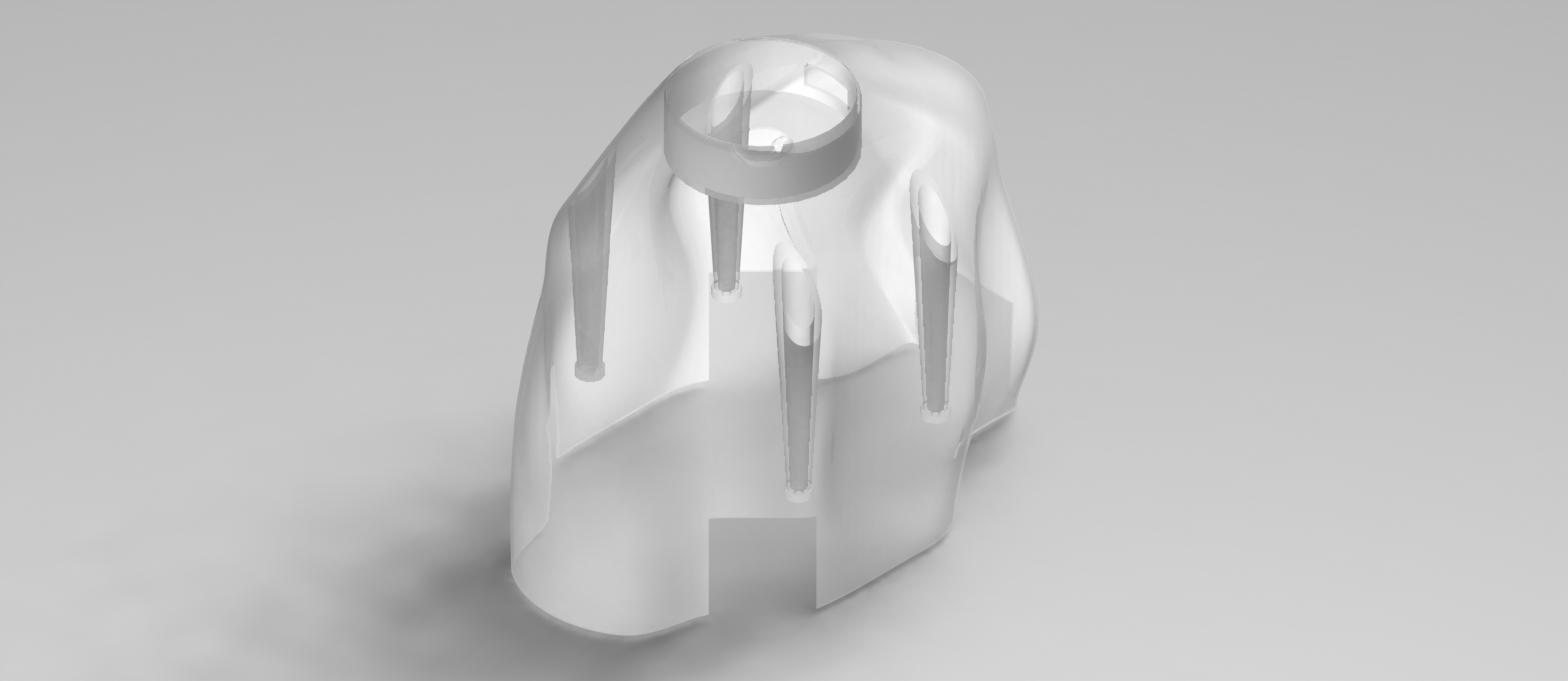
\includegraphics[width=\textwidth]{Figures/hardware/cover_transPlastic.JPG}
    \caption{Cover rendered using a transparent plastic material. This shows the legs for the attaching the cover to the frame (using screws M2), the cavity for the GPS on the top and the holes on the bottom part for the arms and the battery.}
    \label{fig:hw_cover}
\end{figure}

Finally the GPS-Frame attachment is a 12mm x 12mm and 14mm height that is placed inside the cover, on the bottom whole for the GPS and attach it to the frame with a screw as shown in Figure \ref{fig:hw_gps}.

\begin{figure}[!ht]
    \centering
    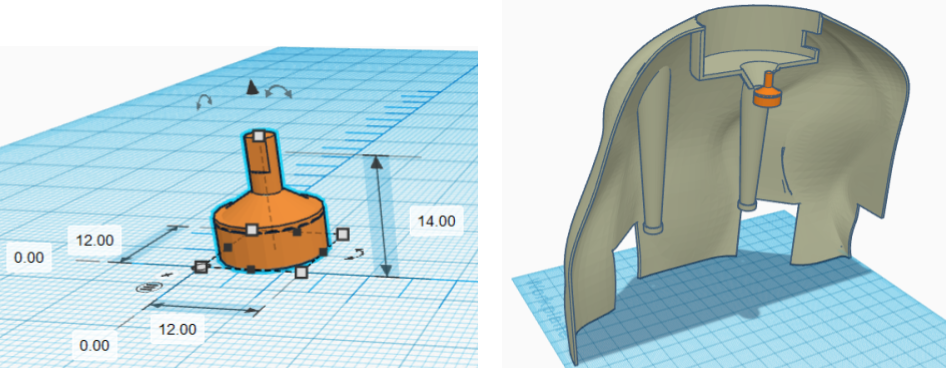
\includegraphics[width=\textwidth]{Figures/hardware/GPS_Attach.png}
    \caption{GPS-Frame attachment dimensions (left) and its placement in the cover (right). This part is held inside the GPS with a screw M1.}
    \label{fig:hw_gps}
\end{figure}

\vfill % <- use this to avoid big blank spaces
\clearpage
%% ========================== ELECTRONICS ==========================
\newpage
\section{Electrical and electronics design}\label{sec:hw_elec}

\subsection{Design overview}
In both modes A and B, the battery provides a power supply of +12V and it is connected to the ESCs. Also both models have in common that all the other components and FPGA board require a power supply for +5V.
In case of Model-A, the +5V supply comes from the ESCs. However, in case of Model-B the +5V is given by the power module, which is between the battery and the the ESCs. 

The next two Figures \ref{fig:hw_modelA} and \ref{fig:hw_modelB} show the hardware diagrams for both models, including the power distribution, the components listed previously in Tables \ref{tab:comp_common} and \ref{tab:comp_AB} and the type of communication between the components and the FPGA.

\begin{figure}[!htb]
    \centering
    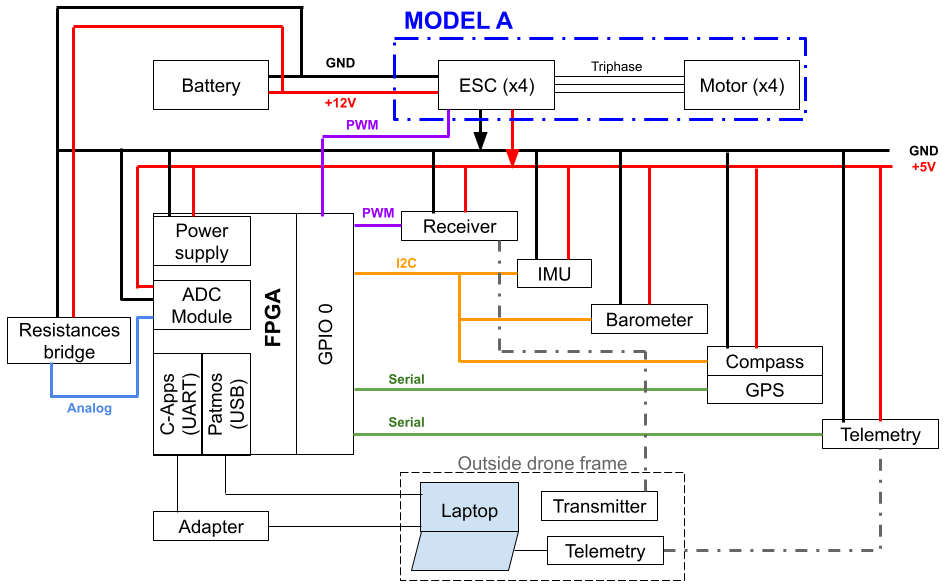
\includegraphics[scale=0.42]{Figures/hardware/Hardware_diagramA_ADC.png}
    \caption{Hardware diagram overview for Model-A.}
    \label{fig:hw_modelA}
\end{figure}

\begin{figure}[!htb]
    \centering
    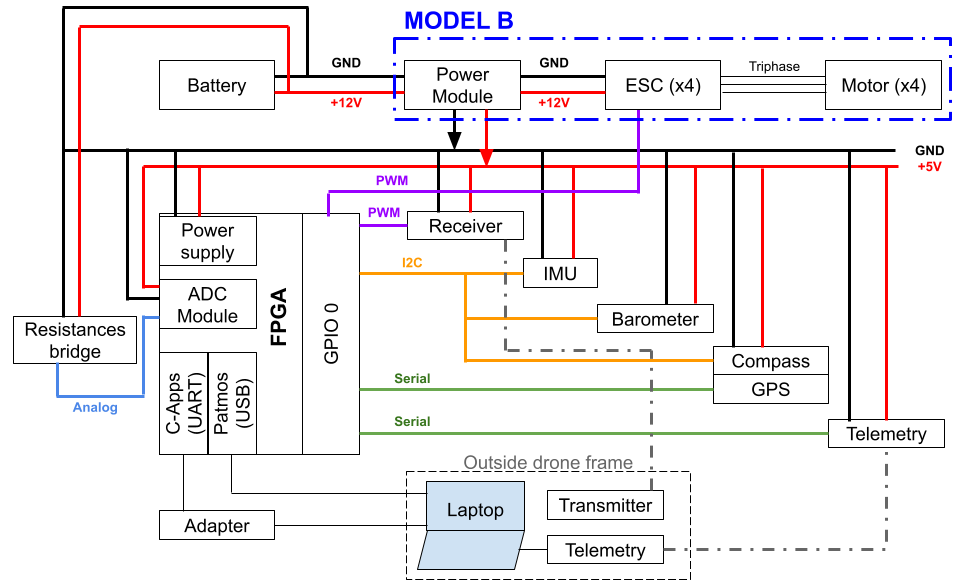
\includegraphics[scale=0.42]{Figures/hardware/Hardware_diagramB_ADC.png}
    \caption{Hardware diagram overview for Model-B.}
    \label{fig:hw_modelB}
\end{figure}

Low-level characteristics of these designs to take into account for the FPGA set-up:
\begin{itemize}
    \item PWM signals from the receiver are inputs, PWM signals going to the ESCs are outputs.
    \item Serial devices have an input (RX) and an output (TX).
    \item The ADC module is a SPI LTC2308 module already integrated within the FPGA. The analog input that it can read is on differential configuration, which has a range of $[+2.048,$ $-2.048]V$. The resistances bridge re-scales the amplitude of the battery $[+11.4,0]V$ to $[+1.937,0]V$, which is safer for the module, as shown in Figure \ref{fig:hw_adc}.
\end{itemize}

\begin{figure}[H]
    \centering
    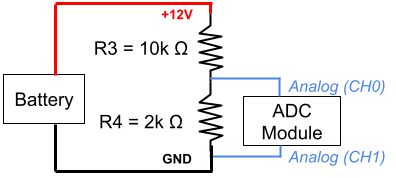
\includegraphics[scale=0.45]{Figures/hardware/resistances_bridge.png}
    \caption{Resistances bridge for the ADC module input. Original design and names from Joop Brokking \cite{bib:brooking}.}
    \label{fig:hw_adc}
\end{figure}

\subsection{FPGA and PCB}

Going into more detail on the electronics design, the following Figure \ref{fig:hw_pins} shows the pins connection of the FPGA to the devices. This diagram is the same for both models.

\begin{figure}[!ht]
    \centering
    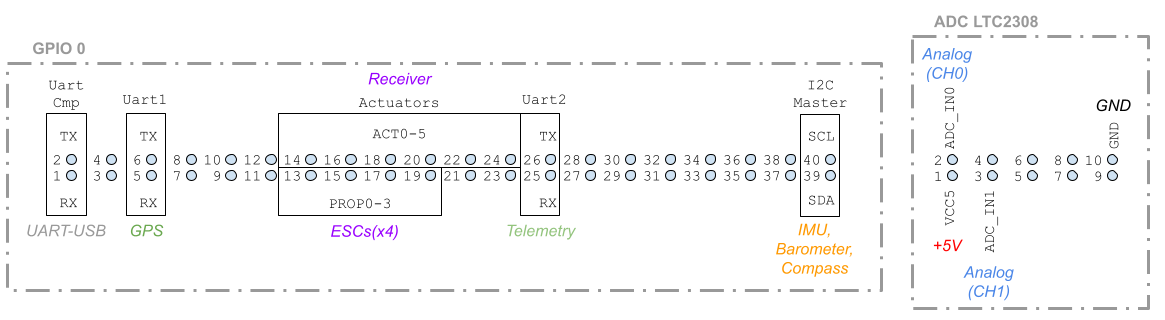
\includegraphics[width=\textwidth]{Figures/hardware/FPGA_pins_ADC.png}
    \caption{De10-Nano pins connection to the components. The pins on use have their name next to them and they are contained in a box with the name of the device type (written in black: UART1, I2CMaster,...) and what physical component is (written in the same color as in the global diagram in Figures \ref{fig:hw_modelA} and \ref{fig:hw_modelB}: receiver, GPS, compass,...)}
    \label{fig:hw_pins}
\end{figure}

In order to simplify the assembly and reduce the amount of wiring in the frame, a PCB was designed for this project.
The PCB was designed in an open source software called DipTrace using the mechanical layout of De10-Nano board as shown in Fig. \ref{fig:mech_layout}. It was designed as a shield for the FPGA. The shield is attached to the GPIO pins and the analog pins of the FPGA and it is fixed by bolting it on 4 corners. The complete PCB design can be seen in Fig. \ref{fig:pcb}.  The PCB remains the same for both model drones i.e. Model A and B and the only difference being that in the model B, the 5V power comes from a power module and it slots into Model B pins in the PCB shield. Whereas in a Model A, the power is directly received from ESC through a Battery Elimination Circuit (BEC). The convention for the pin hole design is such that, the square pins are for power and the circular holes are for other pins.

\begin{figure}[!htb]
    \centering
    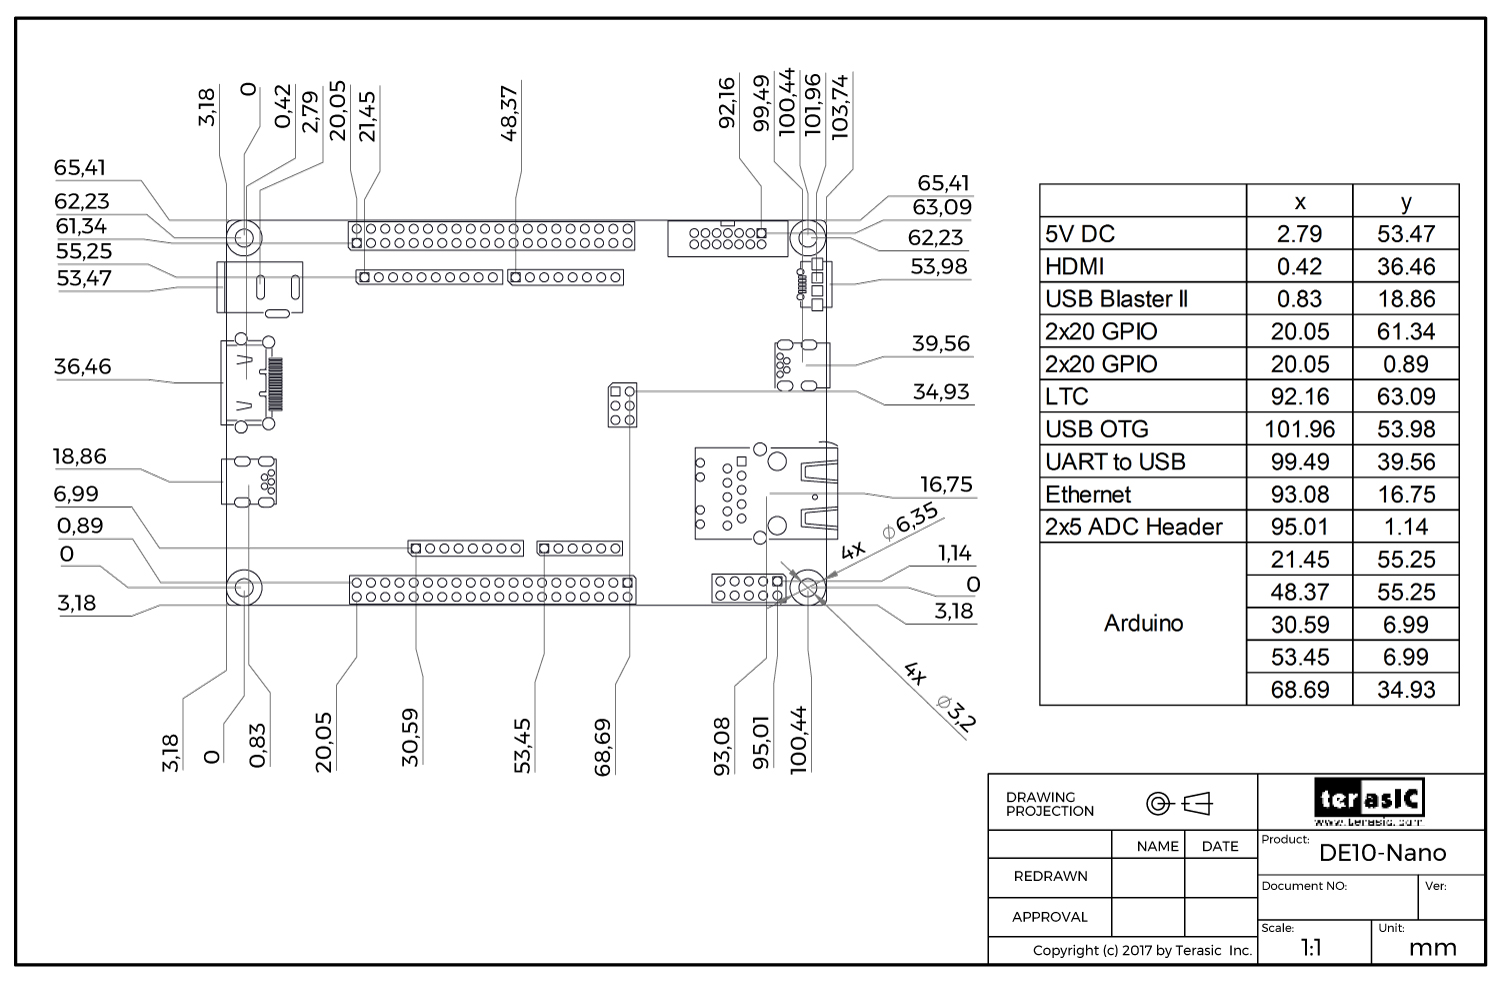
\includegraphics[width=\textwidth]{Figures/hardware/mechanical_layout.jpg}
    \caption{The mechanical layout of the De10-Nano board \cite{bib:fpga_layout}.}
    \label{fig:mech_layout}
\end{figure}

\begin{figure}[!htb]
    \centering
    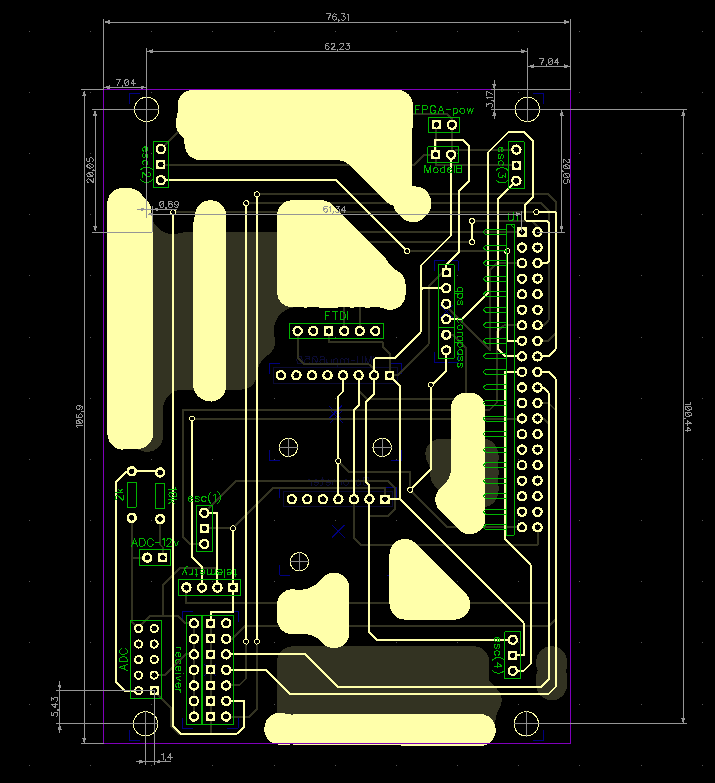
\includegraphics[width=\textwidth]{Figures/hardware/PCB_diptrace.PNG}
    \caption{Top view of the PCB shield designed for de10-nano board.}
    \label{fig:pcb}
\end{figure}

\chapter{Flight Controller Design}\label{ch:sw}
The flight controller developed is a control structure for stabilization of a quad-rotor. The flight controller takes data from different sensors to get the position and orientation of the drone and uses a Proportional Integral and Derivative (PID) control to stabilize the drone. It is developed is based on the YMFC-AL and YMFC-32 projects by Joop Brokking \cite{bib:brooking}, where the author develops a fight controller for an Arduino Uno and STM32 board. This project was translated to C language and configured to work with De10-Nano with necessary libraries \cite{bib:gpsLib} \cite{bib:tu_viena}.
The fight-controller developed has multiple functionalities apart from stabilization and this requires a 6-channel transmitter to switch to different modes. Channel 1-4 are used to control the quad copter movements which are throttle, roll, pitch and yaw respectively. Channel 6 is used lock heading of the drone to one direction also known as holonomic motion. Whereas the channel 5 is used to control the mode of flight which are:
\begin{itemize}
    \item Manual mode- for 0-1200 pulse width 
    \item Altitude hold mode- for 1200-1600 pulse width 
    \item Position hold mode- for 1600-1950 pulse width 
    \item Return To Home- for greater than 1950 pulse width
\end{itemize}
These modes are further explained in detail in Sec. \ref{sec:general_working}.
The above defined modes are possible by receiving different data from different sensors attached to the drone such as:
\begin{itemize}
    \item Inertial Measurement Unit (IMU) - to provide the drone's orientation data i.e. the pitch, roll and yaw angles
    \item Barometer - To provide the altitude at which the drone is flying
    \item Global Positioning System (GPS)- to provide the global positioning of the drone
    \item Compass - to provide the absolute heading of the drone.
    \item Telemetry - To send and receive data from the drone during its flight
    \item ADC module - To convert battery voltage to digital values for drone stabilization
    \item FTDI -  To upload a program to the FPGA board.
    \item Electronic Speed Controller (ESC) - It is used to control the brushless DC motors using PWM signals
\end{itemize}

\section{General Working}\label{sec:general_working}
The flight controller works on a multi-core architecture with 4 parallel cores, where the PID controller, LED devices and analog read run on main core which is core-0; the I2C devices like, compass, IMU, Barometer run on core-1; the PWM signals devices like ESCs and RF- receiver are in core-2; the UART devices like GPS and Telemetry are in core-3. All the cores run at 50Hz whereas the GPS runs are a slower speed due to time it takes to read the data.

The Flight controller program receives the orientation data from IMU and compass, altitude data from Barometer, position data from GPS, Battery voltage from analog pins of the FPGA. The data from IMU, barometer, compass and GPS are provided as feedback to the PID controller, which controls the drone in different modes. Additionally, the supplied voltage from the battery decreases overtime during the flight of the drone. To compensate this, the battery voltage is read from the ADC module and it is used to correct the output for the motors as seen from Fig. \ref{fig:flight_controller}. A test code for battery voltage calculator module was developed \ref{ch:test}, but this functionality was not implemented together with the final version of the flight controller code due to time constraints.

\begin{figure} [H]
    \centering
    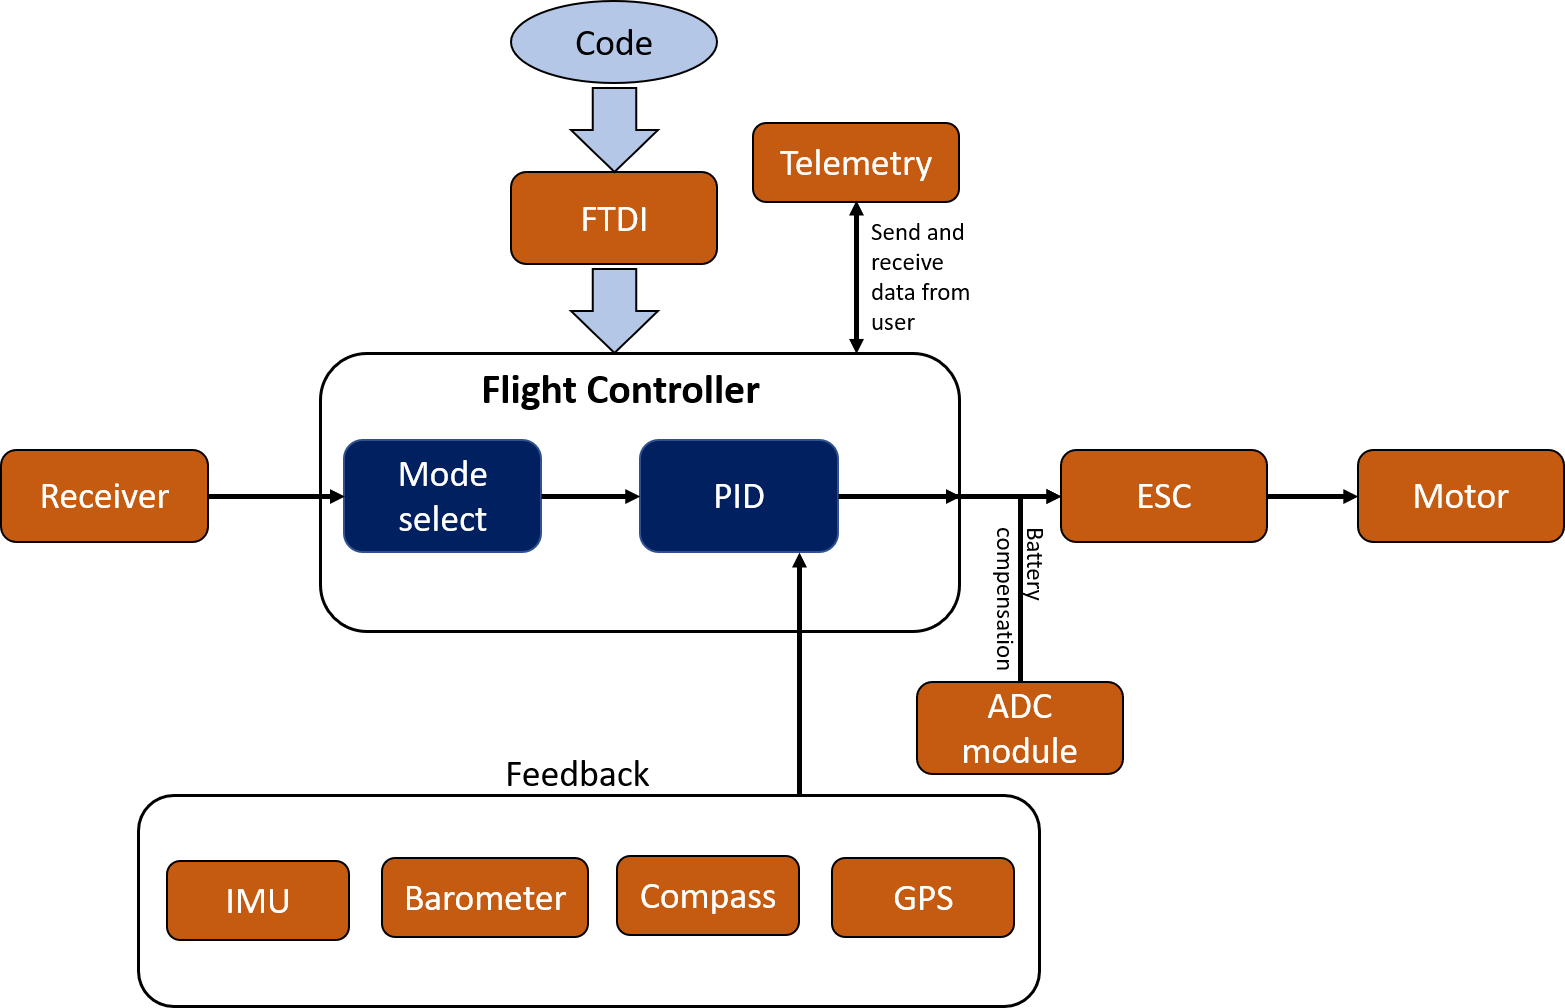
\includegraphics[width=\textwidth]{Figures/implementation/flight_controller.png}
    \caption{Overview of Flight controller model}
    \label{fig:flight_controller}
\end{figure}

Working of different modes:
\subsection{Manual mode}\label{subsec:manual_control}
Manual mode is used to navigate the drone using a transmitter controlled by a pilot. It is achieved only by using an IMU. The controller calculates the motor pwm signals based on the input from the IMU and the RF-transmitter. This is then fed to the esc of the respective motors to control the pitch, roll and yaw of the drone. This functionality has been tested and is its PID gains are fined tuned for stabilization.
\subsection{Altitude hold}\label{subsec:altitude_hold}
Altitude hold mode is to make the drone hover at a constant altitude. This mode is achieved using an IMU and a barometer, where the IMU does the same functions as mentioned in Sub-section \ref{subsec:manual_control} and barometer data is used to control the throttle of all the motors to achieve altitude stabilization. This functionality was tested to output proper results, but the PID gains were not properly tuned due to time constraints.
\subsection{Position hold}\label{subsec:position_hold}
Position hold mode is to make the drone hover and stay fixed at a certain position provided. This mode is achieved using an IMU, compass, barometer and a GPS, where the GPS and compass, provides the position and absolute heading information of the drone and this is used to control the drone to remain at a fixed position. This functionality has not been tested due to low frequency of GPS data, and issues regarding core-3 hanging. Information regarding core-3 issues is explained in Chapter \ref{ch:concl}.
\subsection{Return To Home}\label{subsec:rth}
The drone records the home position at the beginning and when this mode is switched on, it return back to the recorded home location. This mode also, uses IMU, compass, Barometer and GPS to achieve this task. Similarly, due to the issues regarding core-3, this functionality has not been tested.

























\chapter{Implementation}\label{ch:impl}

\section{Built drones}

In total, four full-assembled drones were built for this project using the hardware described in Chapter \ref{ch:hw}: two model-A units and two model-B, both models shown in Figures \ref{fig:imp_models_noCover} and \ref{fig:imp_modelsFULL}. The four drones are shown in Figure \ref{fig:imp_4drones}, and they are separated in two groups: the drones that belong to AAU (one model-A and one model-B) and the ones that belong to DTU (also one model-A and one model-B). Each group of drones has a single transmitter, that can be paired with any receiver of the drones.

Additionally, there are two not-assembled spare sets and each set has a FPGA, a PCB, a cover, a FPGA-frame attachment, a frame and the sensors that are attached on top of the PCB.


\begin{figure} [H]
    \centering
    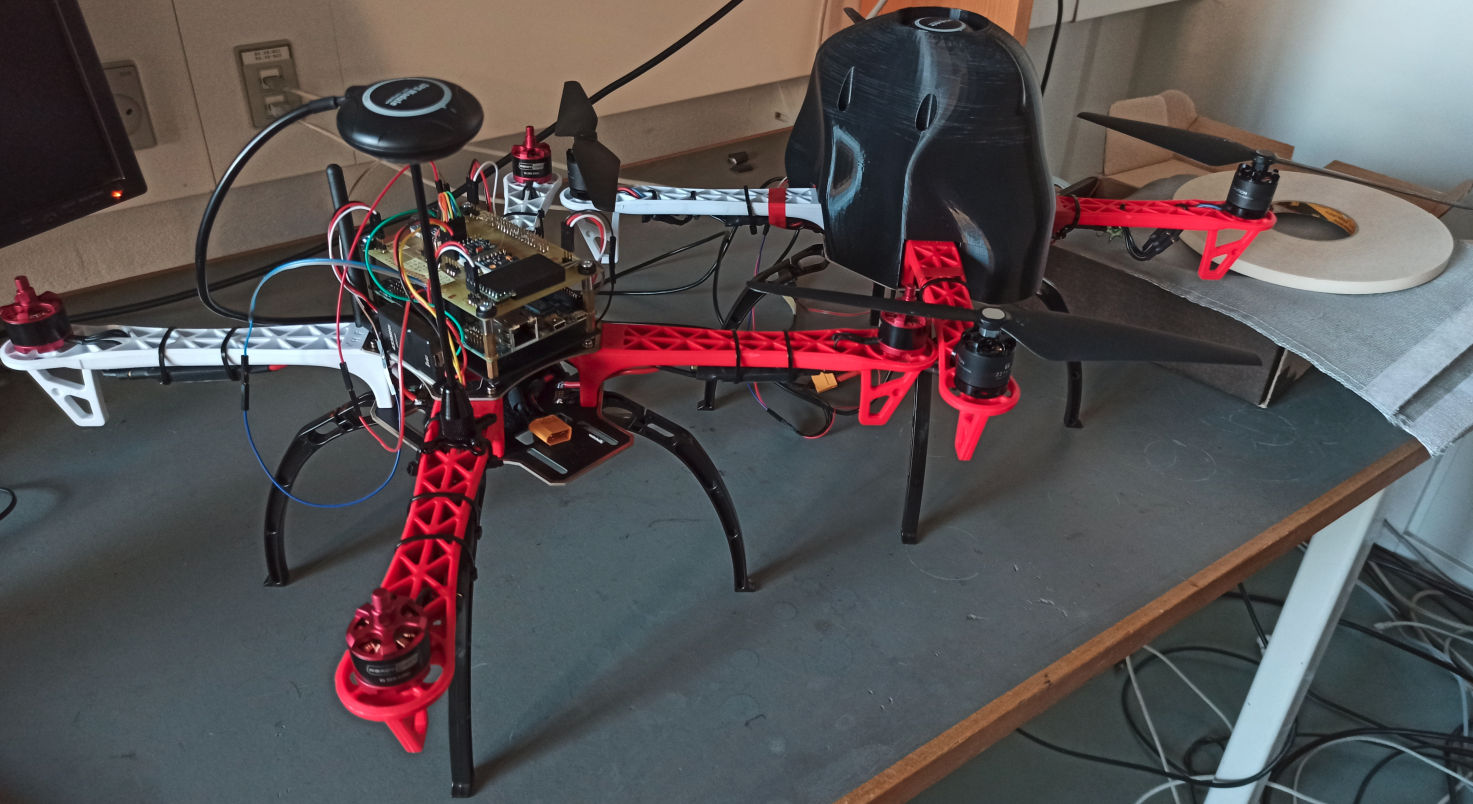
\includegraphics[width=\textwidth]{Figures/implementation/modelA_and_B.png}
    \caption{Model-A without cover (left) and Model-B (right). Both units have inside a FPGA with a PCB attached as shown.}
    \label{fig:imp_models_noCover}
\end{figure}

\begin{figure} [H]
    \centering
    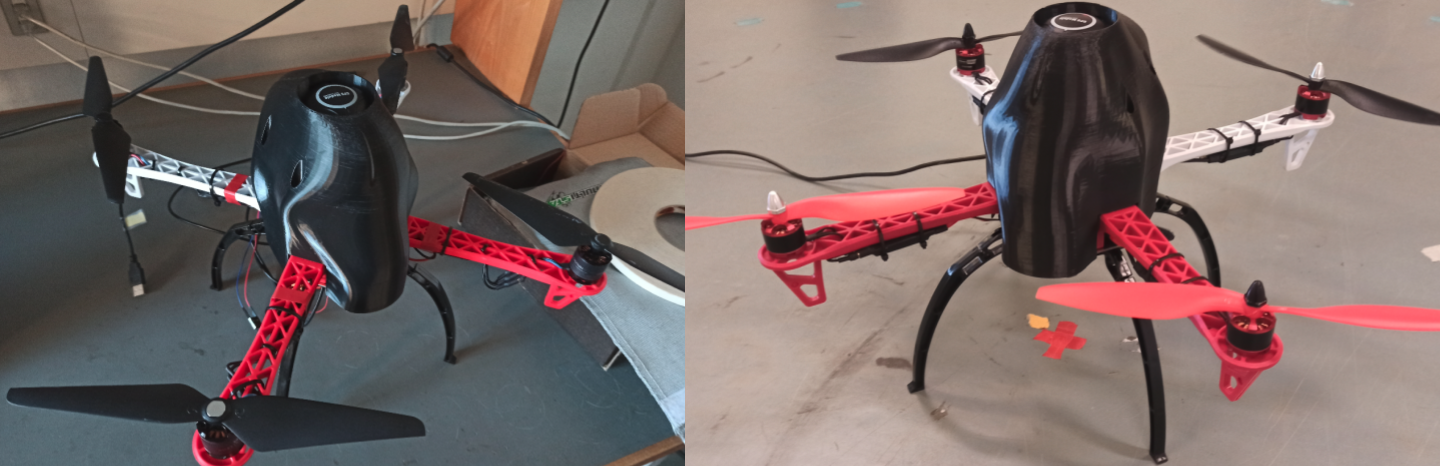
\includegraphics[width=\textwidth]{Figures/implementation/modelA_and_B_assembled.png}
    \caption{Fully assembled Model-B (left) and A (right) units.}
    \label{fig:imp_modelsFULL}
\end{figure}


\begin{figure} [H]
    \centering
    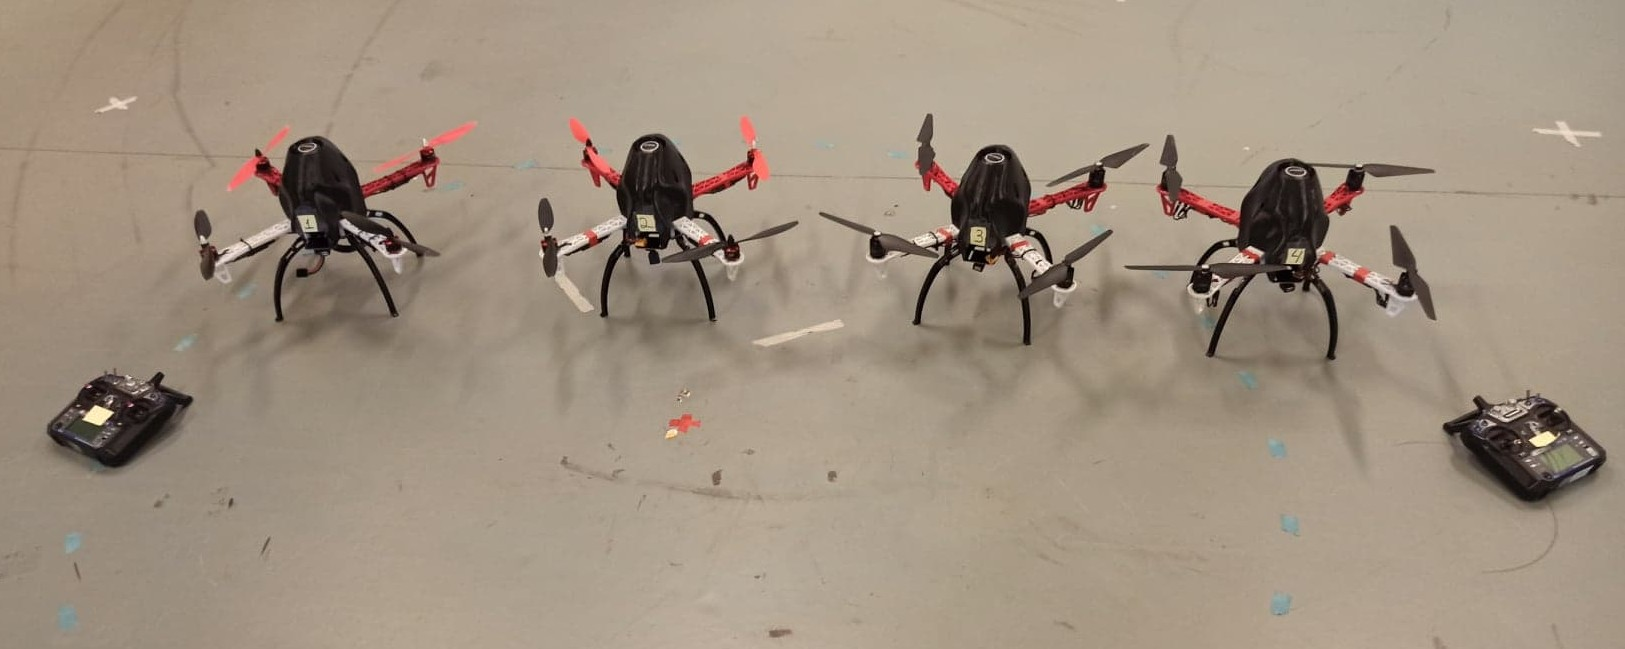
\includegraphics[width=\textwidth]{Figures/implementation/four_drones_tel.jpg}
    \caption{From left to right: AAU transmitter, drone 1 (Model-A, group AAU), drone 2 (Model-A, group DTU), drone 3 (Model-B, group AAU), drone 4 (Model-B, group DTU), DTU transmitter. Next to each drone, there is its paired telemetry module for a remote station.}
    \label{fig:imp_4drones}
\end{figure}


\section{Patmos configuration}

The Patmos architecture for this project is called de10-nano-drone and its configuration is quite different from the standard de10-nano or the default configurations. Here are some its hardware specifications:

\begin{itemize}
    \item ADC Module: This resource is available inside the FPGA and hard-wired to it. This module has its own set of pins for the analog inputs and its separate power supply.
    \item I2C Master for multiple sensors: the SDA and SCL pins work as a bus to connect three different sensors (IMU, barometer, compass).
    \item Second and third UART ports: the second UART has the same baud rate as the GPS and the third UART has the same baud rate as the telemetry module and a bigger FIFO depth for longer messages exchange.
    \item Modification on Actuators: it works as an input and it has 6 pins, so it is used for the 6-channels receiver.
    \item External memory of 1GB: it uses the micro SD card from the FPGA. This is required for the multi-core feature.
    \item Multi-core assignment: there are 4 cores in use and the devices must be assigned to a core (by default they are assigned to core nr.0). The devices have been assigned as it follows:
    \begin{itemize}
        \item Core 0: ADC module and LEDs.
        \item Core 1: I2C master.
        \item Core 2: Actuators (receiver), and this also includes Propulsion (motors).
        \item Core 3: UART 2 and 3.
    \end{itemize}
\end{itemize}


\section{Software architecture}

The flight controller algorithm and functionalities described on the previous Chapter \ref{ch:sw} have been implemented as an application written in C. This implementation is divided in different groups of scripts and header files. As shown in Figure \ref{fig:imp_arch}, there are six groups:

\begin{itemize}
    \item Basic functionalities: it contains all the low-level and hardware-related dependencies.
    \item Components: using the basic functionalities, it implements the full functionalities of the devices and they are meant for the specific components from the Tables \ref{tab:comp_common} and \ref{tab:comp_AB}.
    \item Flying functionalities and flight controller: they contain the different modes and the flight algorithm described on Section \ref{sec:general_working}.
    \item Test programs: it implements different test scripts for checking the functionality of every device. Every program is described in Chapter \ref{ch:test}.
    \item Simulation: it contains the simulation scripts, dependencies and simulation scenes, which are described in Section \ref{sec:simulation}
\end{itemize}

\begin{figure} [H]
    \centering
    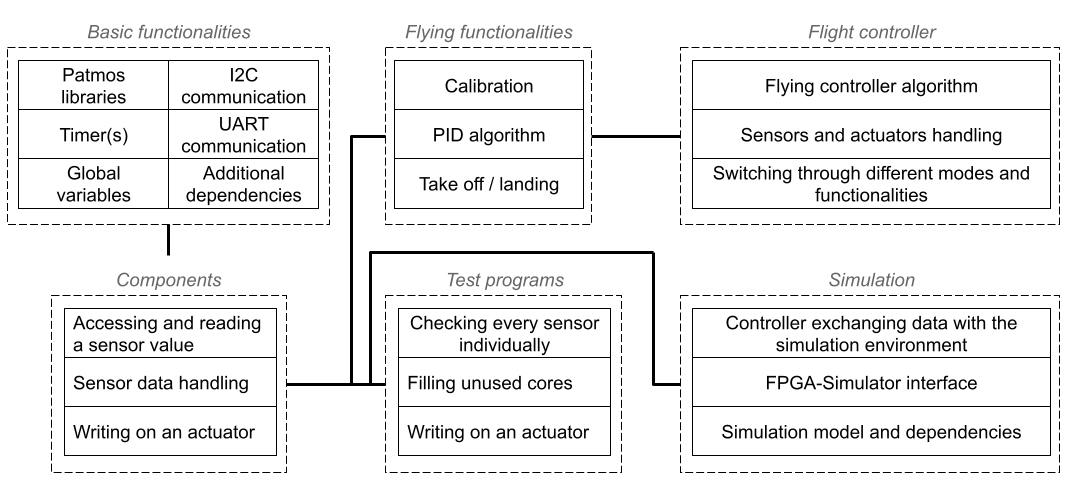
\includegraphics[width=\textwidth]{Figures/implementation/fc_architecture.png}
    \caption{Software architecture for the flight controller and additional functionalities.}
    \label{fig:imp_arch}
\end{figure}

%\vfill % <- use this to avoid big blank spaces
%\clearpage
%\newpage
% Start on a new page
\section{Drone simulation}\label{sec:simulation}

Another concept for the project was to develop a simulation model of the drone that can be used for testing the flight controller while running on the FPGA. The main idea for this approach is shown in Figure \ref{fig:sim_concept} and it can be described as follows:

\begin{itemize}
    \item The goal is to simulate and find bugs on the flight controller, so the simulation aims to test the drone on the fly and how it reacts to changes on the commands from the pilot through the transmitter. Thus the actual FPGA, receiver and transmitter are needed, as shown in Figure \ref{fig:sim_setup}.
    
    \item The Patmos architecture and a modified version of the flight controller are downloaded on the board.
    
    \item The modified version of the flight controller uses the telemetry port to exchange messages with the simulator. It gets all the sensors values required (IMU, barometer, GPS,...) from the messages instead of using their normal ports (I2C, UART1).
    
    \item On the PC Station, it is needed a program that works as an interface between the FPGA and the simulator, which was implemented as a Python script. This interface access the port where the UART2 is sending/receiving messages and the simulation drone. In the run, it gets the sensors values, converts them to the same format as the real ones and sends them to the FPGA. On the other hand, it gets the motor commands from the FPGA and converts them into the units that the simulation drone works with (in this case $rad/s$) and sends it to the simulation.
    
\end{itemize}

\begin{figure} [H]
    \centering
    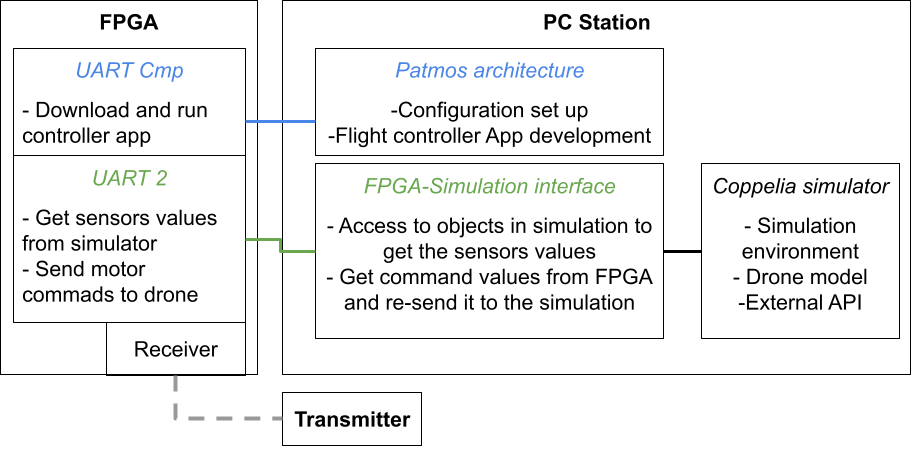
\includegraphics[width=\textwidth]{Figures/simulation/simulation_concept.png}
    \caption{Simulation diagram}
    \label{fig:sim_concept}
\end{figure}

\begin{figure} [H]
    \centering
    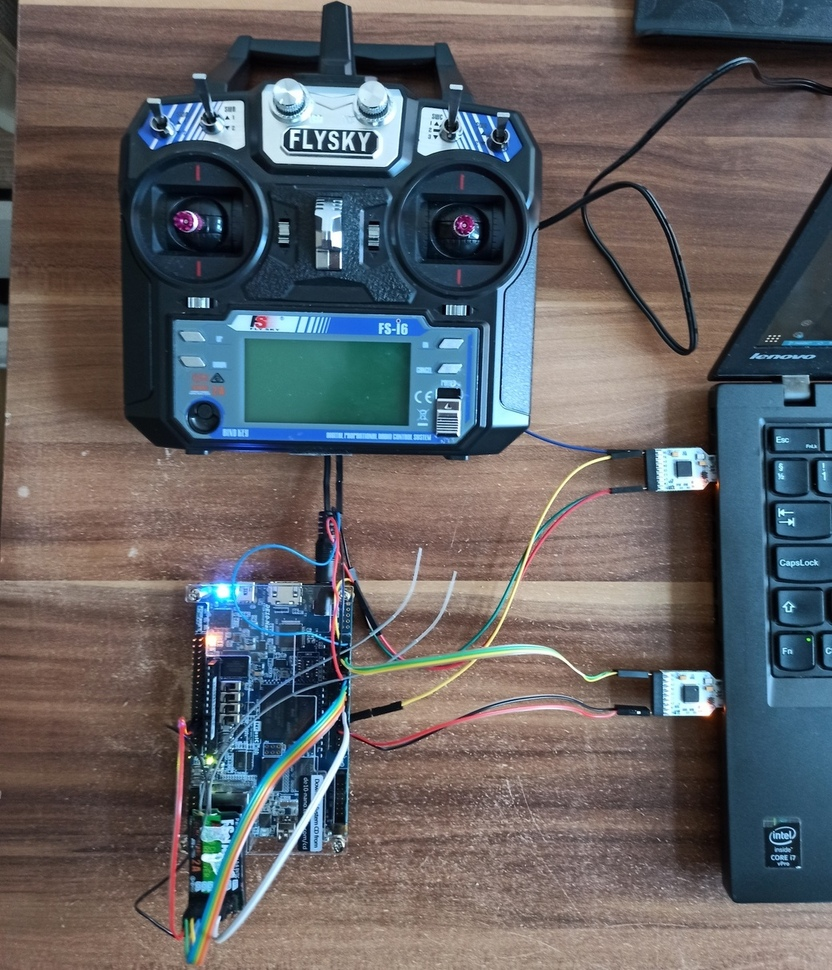
\includegraphics[scale=0.3]{Figures/simulation/simulation_setup.jpg}
    \caption{Simulation set up: transmitter (top left), FPGA with a receiver, two UART-USB adapters (connected to UART Cmp and UART2), and a laptop (right).}
    \label{fig:sim_setup}
\end{figure}

The drone model presented in \ref{sec:hw_mec} can be exported from SolidWorks into Universal Robot Description Format (URDF) \cite{bib:urdfPlugin}. Thus, the simulator chosen is CoppeliaSim, which is compatible with this format.

Both Model-A and Model-B were successfully imported into CoppeliaSim and added to the simulator library as robot models, as shown in Figure \ref{fig:sim_models}. On top of that, the models from Solidworks do not include the sensors and these had to be added manually on the simulated models. A successful test showed that the communication between the different elements was possible and the program interface could exchange messages with the FPGA and get values from the sensors on the simulation.s

However, the CoppeliaSim simulator does not have fluid mechanics on the physics engine, so the simulation environment is on a vacuum space. In order to make a mobile robot move within a 3D space, it is necessary to implement on the simulation scrips the differential equations and forces that must be applied on the body. 

There are another mobile robot models within the models library that have managed to successfully implement this (another quad-copter drone and a swimming snake robot), but this was not achieved for this project. Both drone models were set as dynamic and responsive objects and they can spin their motors, but they cannot take off properly. Finally, this part of the project remains unfinished due to the fact that the real lab and components were accessible.

\begin{figure} [H]
    \centering
    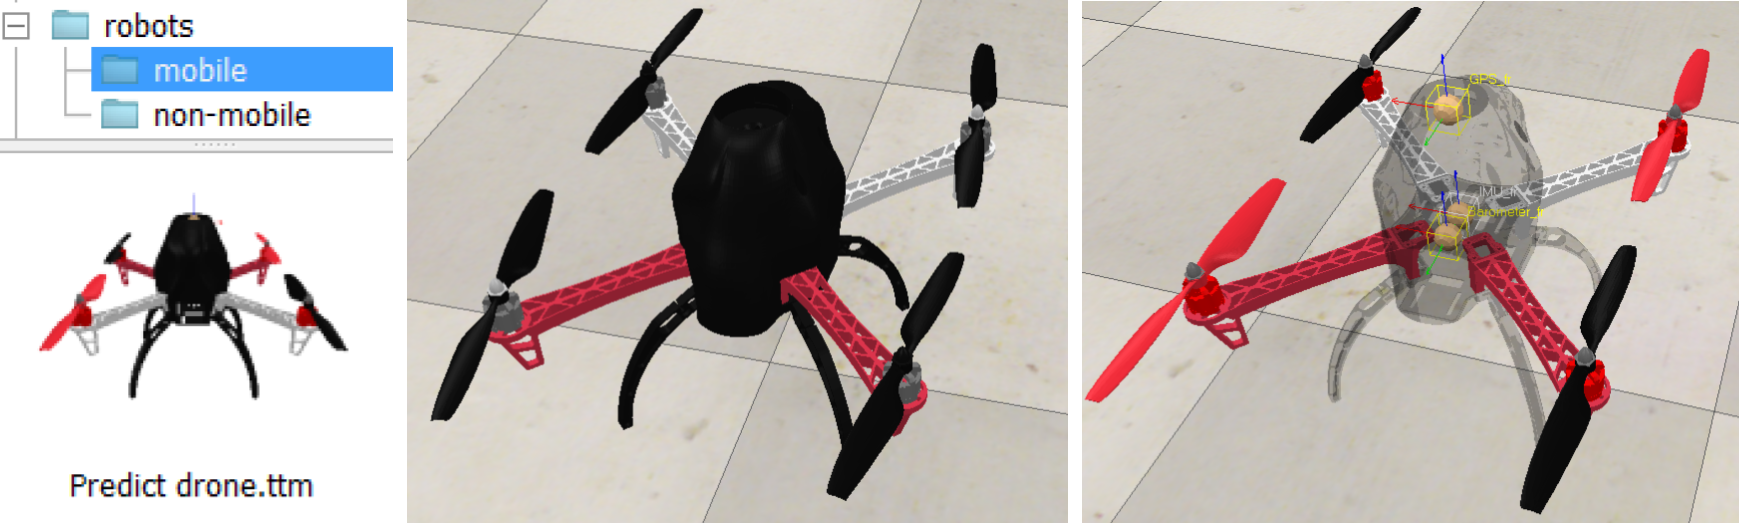
\includegraphics[width=\textwidth]{Figures/simulation/coppelia_model.png}
    \caption{From left to right: drone model imported and saved in Coppelia library, a drone frame in simulation (example with a Model-B), showing the inside of the cover where the sensors had to be added to the simulation model (example with a Model-A).}
    \label{fig:sim_models}
\end{figure}

% where to put this
%%\vfill % <- use this to avoid big blank spaces
%\clearpage
%\newpage
% Start on a new page
\section{Drone simulation}\label{sec:simulation}

Another concept for the project was to develop a simulation model of the drone that can be used for testing the flight controller while running on the FPGA. The main idea for this approach is shown in Figure \ref{fig:sim_concept} and it can be described as follows:

\begin{itemize}
    \item The goal is to simulate and find bugs on the flight controller, so the simulation aims to test the drone on the fly and how it reacts to changes on the commands from the pilot through the transmitter. Thus the actual FPGA, receiver and transmitter are needed, as shown in Figure \ref{fig:sim_setup}.
    
    \item The Patmos architecture and a modified version of the flight controller are downloaded on the board.
    
    \item The modified version of the flight controller uses the telemetry port to exchange messages with the simulator. It gets all the sensors values required (IMU, barometer, GPS,...) from the messages instead of using their normal ports (I2C, UART1).
    
    \item On the PC Station, it is needed a program that works as an interface between the FPGA and the simulator, which was implemented as a Python script. This interface access the port where the UART2 is sending/receiving messages and the simulation drone. In the run, it gets the sensors values, converts them to the same format as the real ones and sends them to the FPGA. On the other hand, it gets the motor commands from the FPGA and converts them into the units that the simulation drone works with (in this case $rad/s$) and sends it to the simulation.
    
\end{itemize}

\begin{figure} [H]
    \centering
    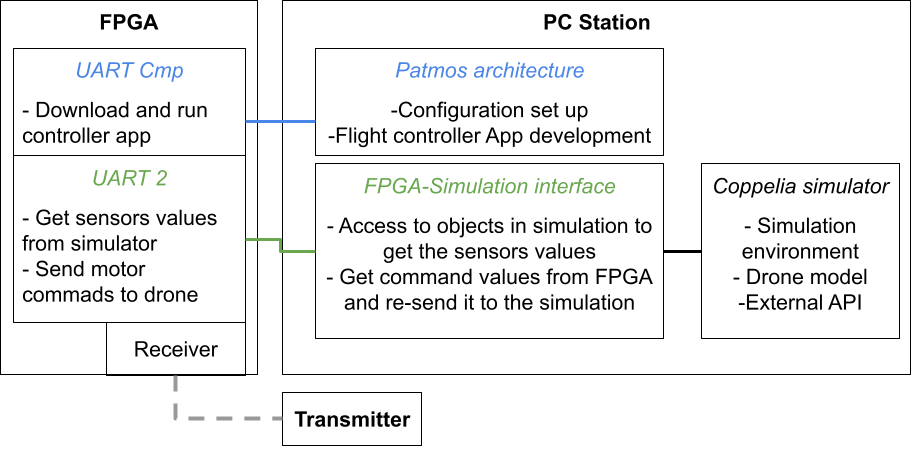
\includegraphics[width=\textwidth]{Figures/simulation/simulation_concept.png}
    \caption{Simulation diagram}
    \label{fig:sim_concept}
\end{figure}

\begin{figure} [H]
    \centering
    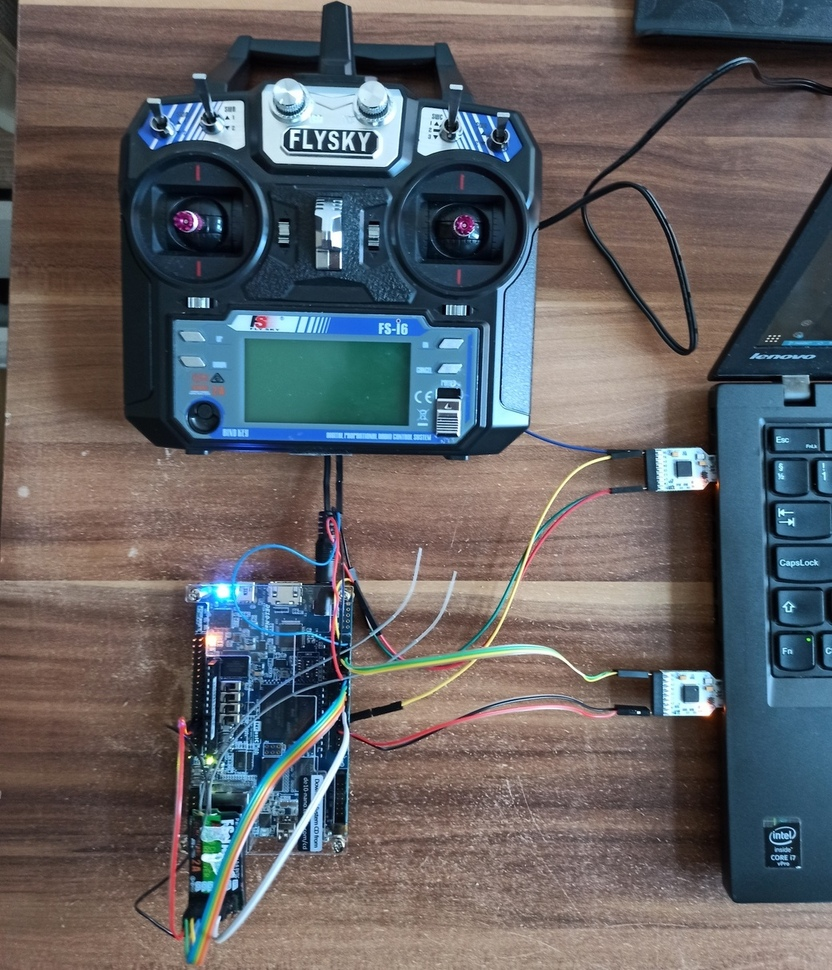
\includegraphics[scale=0.3]{Figures/simulation/simulation_setup.jpg}
    \caption{Simulation set up: transmitter (top left), FPGA with a receiver, two UART-USB adapters (connected to UART Cmp and UART2), and a laptop (right).}
    \label{fig:sim_setup}
\end{figure}

The drone model presented in \ref{sec:hw_mec} can be exported from SolidWorks into Universal Robot Description Format (URDF) \cite{bib:urdfPlugin}. Thus, the simulator chosen is CoppeliaSim, which is compatible with this format.

Both Model-A and Model-B were successfully imported into CoppeliaSim and added to the simulator library as robot models, as shown in Figure \ref{fig:sim_models}. On top of that, the models from Solidworks do not include the sensors and these had to be added manually on the simulated models. A successful test showed that the communication between the different elements was possible and the program interface could exchange messages with the FPGA and get values from the sensors on the simulation.s

However, the CoppeliaSim simulator does not have fluid mechanics on the physics engine, so the simulation environment is on a vacuum space. In order to make a mobile robot move within a 3D space, it is necessary to implement on the simulation scrips the differential equations and forces that must be applied on the body. 

There are another mobile robot models within the models library that have managed to successfully implement this (another quad-copter drone and a swimming snake robot), but this was not achieved for this project. Both drone models were set as dynamic and responsive objects and they can spin their motors, but they cannot take off properly. Finally, this part of the project remains unfinished due to the fact that the real lab and components were accessible.

\begin{figure} [H]
    \centering
    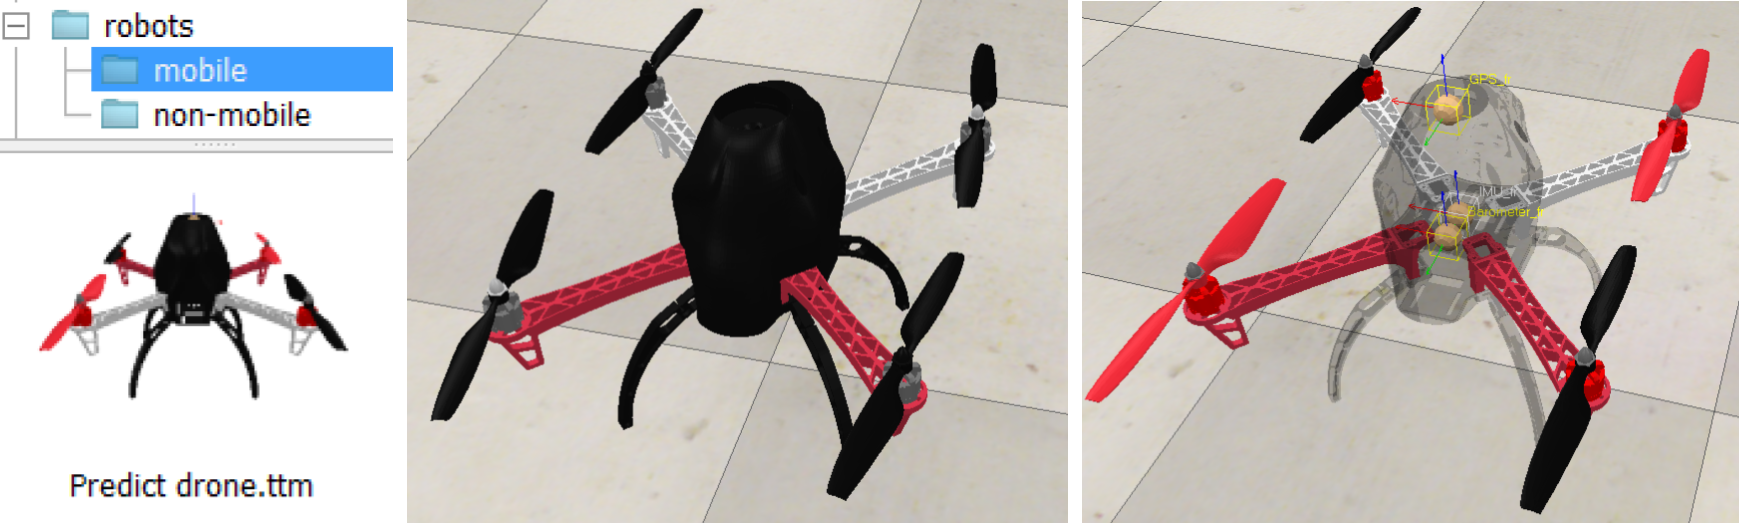
\includegraphics[width=\textwidth]{Figures/simulation/coppelia_model.png}
    \caption{From left to right: drone model imported and saved in Coppelia library, a drone frame in simulation (example with a Model-B), showing the inside of the cover where the sensors had to be added to the simulation model (example with a Model-A).}
    \label{fig:sim_models}
\end{figure}

\chapter{Tests and results}\label{ch:test}
Testing of the drone involves, testing the drone stabilization and hovering its manual control and landing. But before a flight test is done, the drone must be tested  to verify if all its sensors are in order and it also requires an initial calibration of the sensors. The sensors are run in a multi-core architecture, where the i2c devices run on core 1, motors and receivers run on core 2 and GPS and telemetry run on core 3. When running individual sensor tests, dummy functions are introduced to occupy the vacant cores. The tests that are provided for every sensor are as follows:
\begin{enumerate}
    \item Motor test - This test is used to check the direction and the order of the motors as shown in Fig. \ref{fig:motor_direction}. In this test, the motors spin sequentially in an order for 5 seconds each.
     \item ESC calibration test - This test is necessary when a new ESC is used. The 4 ESCs are calibrated to start the motors at 1000$\mu$s pulse and reach its maximum at 2000$\mu$s pulse. This is done by:
     \begin{itemize}
         \item Turn on the transmitter and put the throttle at the maximum position
         \item Switch on the FPGA and upload the program
         \item Wait for the motors to beep 3 times in sets of 3, then lower the throttle of transmitter and wait for the motors to beep again.
         \item Motors are calibrated successfully
     \end{itemize}
    \item IMU test - This test is used to verify the direction and magnitude of pitch, roll and yaw angles of the quad-rotor. The directions of the angles are given in Fig. \ref{fig:imu_angle}. The directions follow right hand thumb rule. Therefore, roll is positive when left wing goes up, pitch is positive when the nose pitches up and yaw is positive when the drone rotates to the right.
    \item Barometer test - This test is used to check the readings of barometer whether they decrease as the drone goes up and increase as the drone descends since, the atmospheric pressure increases with decrease in altitude.
    \item Compass test - This test is used to check the yaw of the drone with respect of the absolute north. The yaw angles are then rounded off to stay in between 0 to 360.
     \item Receiver test - 
     \textit{NOTE: Check if the receiver is paired to transmitter before starting this test [\ref{trans_receiver_pair}]}. 
     This test is used to check if all the channels of the transmitter are being read by the FPGA. The direction and the value limits of the transmitter channels are also calculated and added as transmitter settings to the header file of the Flight controller code. For every channel the minimum, maximum and its middle value are recorded and the direction of the transmitter channel required are displayed in Fig. \ref{fig:tranmitter_direction}. If the direction is opposite to the required direction, the reverse variable of the particular channel is set to 1.
     \item GPS test - This test is used to verify that the GPS has a 3D position lock, i.e. the GPS is locked to more than 8 satellites and displays the current GPS coordinates.
     \item Telemetry test - \textit{NOTE: check is the baud rate for the telemetry is set to 115200 [\ref{telemetry_baud}]}. This test code is used to send and receive telemetry data between different telemetry modules. The test code sends a "hello world" message, and the user runs a python script called  \textit{telemetry\_base} to receive the sent data.
     The test code also contains a code to help tune the PID gains of the motors real time by sending the gain values to the drone wirelessly. This program although can send and receive the gain values, the tuning was unsuccessful real time because, the loop runs at a much lower frequency than the main loop.
     \item Analog test - The test sends a configuration word which specifies how the module has to read the input(either a differential or an absolute input value). In every iteration it changes the module configuration word, so the test program obtains a read from all the analog input pins on the ADC in differential and absolute modes.
\end{enumerate}

\begin{figure} [ht]
    \centering
    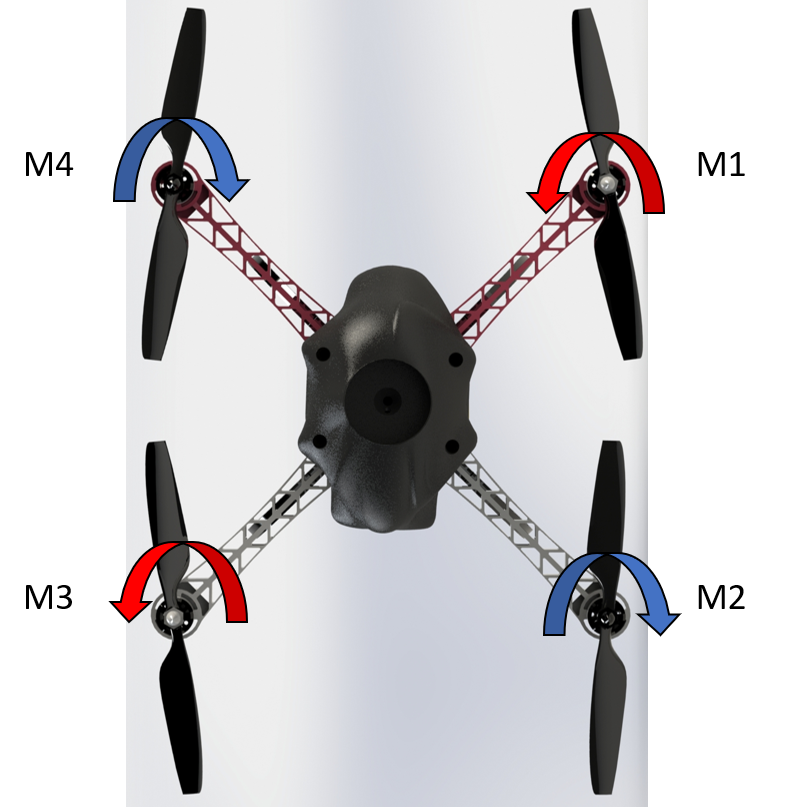
\includegraphics[width=0.5\textwidth]{Figures/testing/motor_directions.png}
    \caption{Directions and order of the motor Assembly}
    \label{fig:motor_direction}
\end{figure}

\begin{figure} [ht]
    \centering
    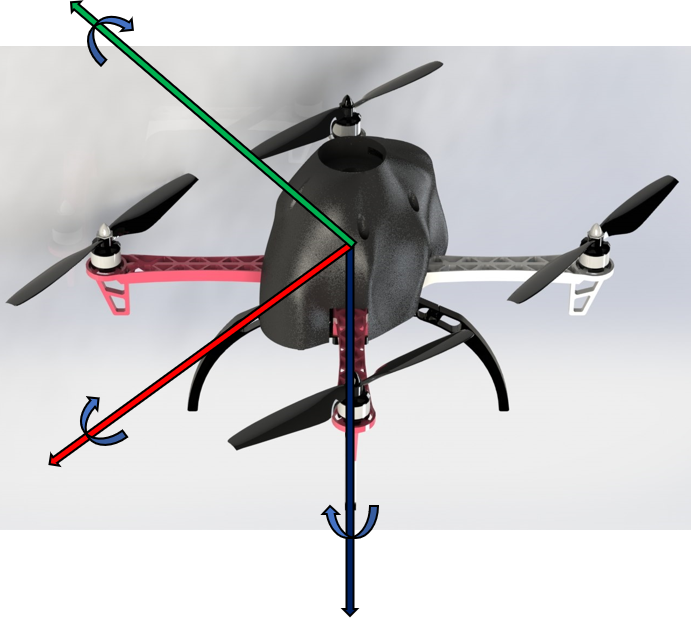
\includegraphics[width=0.5\textwidth]{Figures/testing/imu_directions.png}
    \caption{Roll (X axis, on red), pitch (Y axis, on green) and yaw (Z axis, on black) angles, and the directions of the drone.}
    \label{fig:imu_angle}
\end{figure}

\begin{figure} [ht]
    \centering
    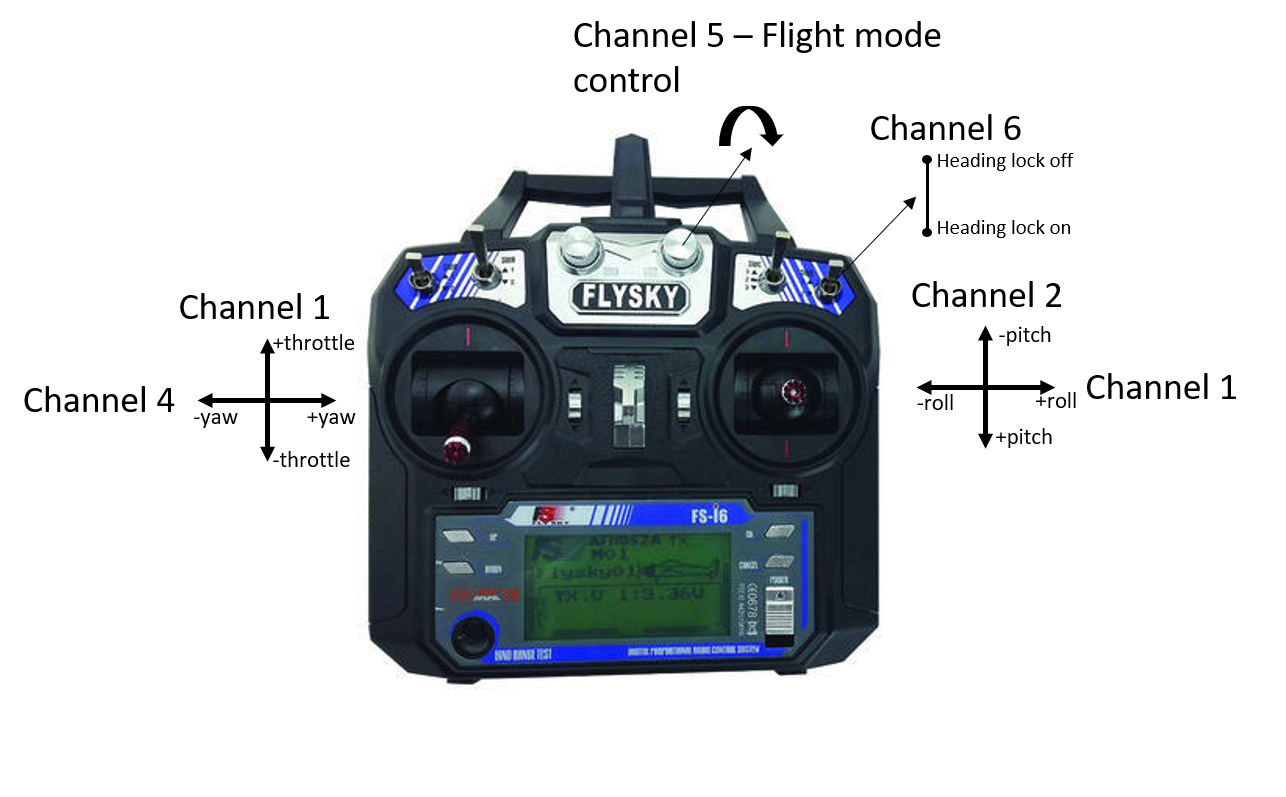
\includegraphics[width=0.5\textwidth]{Figures/testing/transmitter_controls.png}
    \caption{The configurations of a 6-channel transmitter}
    \label{fig:tranmitter_direction}
\end{figure}

After the sensors have been tested, it is necessary to tune the PID values of roll, pitch and yaw angles.



\section{PID tuning test}\label{app:tuning}
The PID tuning procedure is followed as described in \cite{bib:brooking}. The PID gains are tuned while holding the drone at hovering throttle:
\begin{enumerate}
    \item The drone is kept on a flat ground (preferably on grass or carpet) and the initial yaw PID values are set to $K_P=1$,$K_D=0.001$ and $K_i=0$ so as to prevent the drone from rotating while tuning roll and pitch.
    \item The roll and pitch are assumed to have similar gains. The $K_P$ and $K_i$ values are set to 0 and only $K_D$ is varied. 
    \item This values is increased until the drone just becomes restless. The final $K_D$ is taken as 75\% of the current value.
    \item The $K_P$ gain is now increased in steps of 0.2 until it just begins to oscillate. The final $K_P$ is taken as 50\% of the current value.
    \item Similarly, the $K_i$ gain is increased in steps of 0.0001 until it just begins to oscillate. The final $K_i$ is taken as 50\% of the current value.
\end{enumerate} 


\section{Flight test}
Once the PID values are tuned, the manual control of the drone is tested. The test was done in the Vicon lab at AAU. The drone was made to takeoff and the motions of the drone was controlled using a transmitter as seen in Figures \ref{fig:test_floor} and \ref{fig:test_fly}.

Although the barometer sensor was tested for altitude hold mode, the altitude PID values were not tuned due to time constraints. Due to this, the drone takes off and can be controlled but cannot be used in hover mode. Also due to the same reason, it gets difficult while landing the drone. But the cover protects the components from being damaged and due to the height of the cover, it also protects the propellers from over damage as seen in Figure \ref{fig:test_lmao}.

\begin{figure} [!ht]
    \centering
    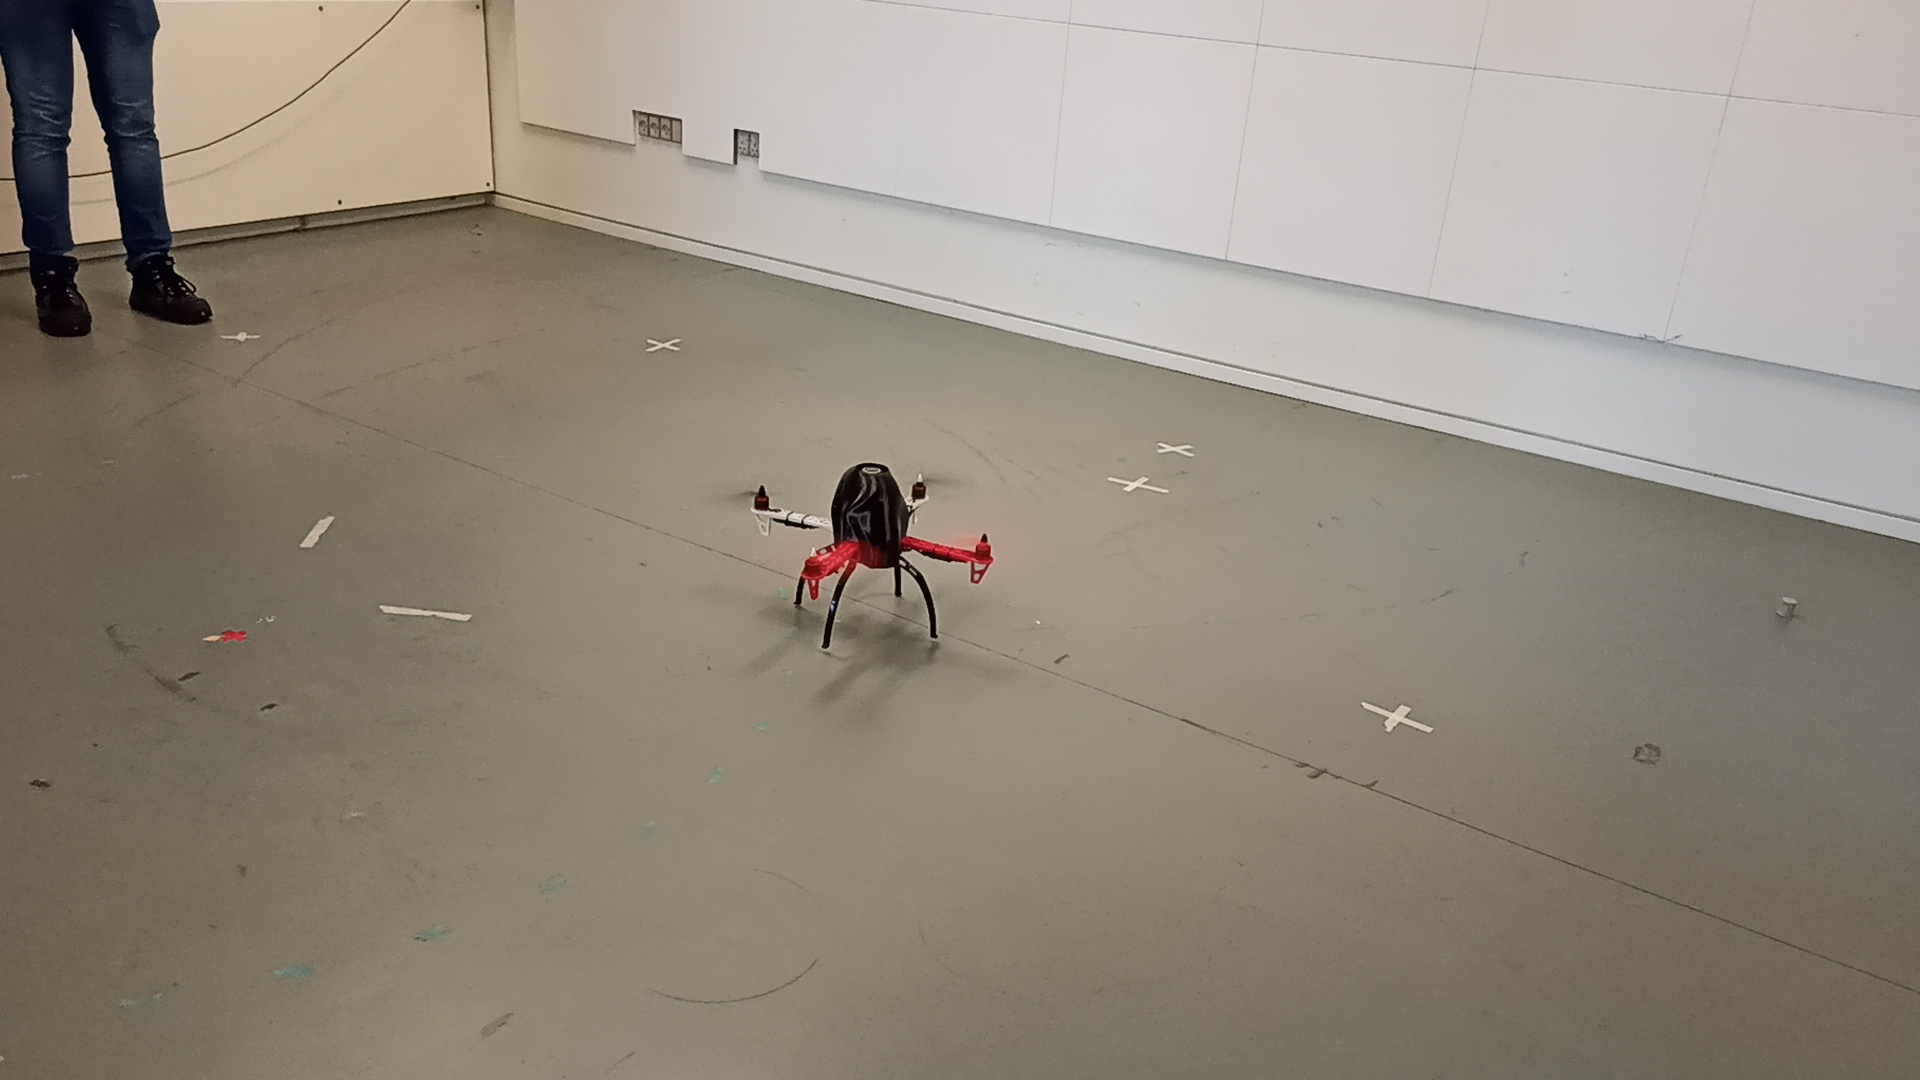
\includegraphics[width=\textwidth]{Figures/testing/drone_floor.jpg}
    \caption{Drone 1 (Model-A) about to take off}
    \label{fig:test_floor}
\end{figure}


\begin{figure} [!ht]
    \centering
    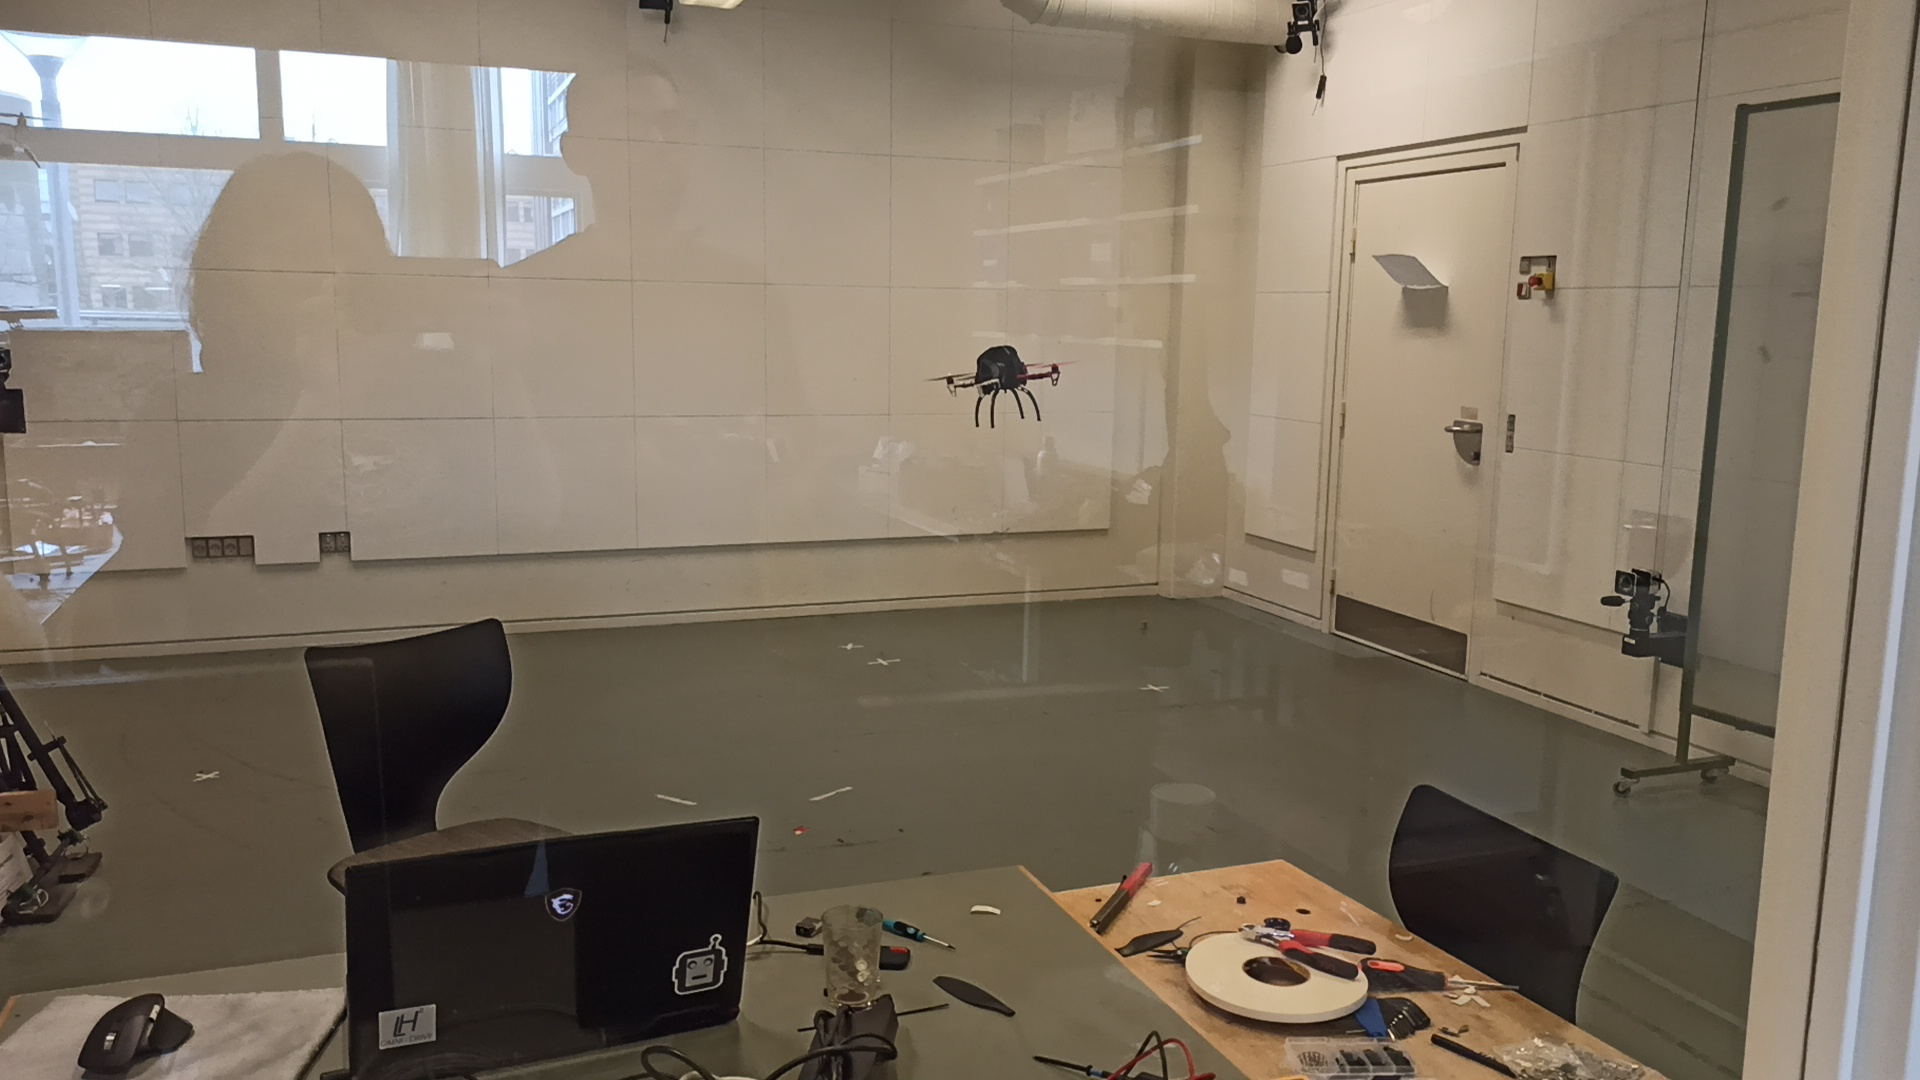
\includegraphics[width=\textwidth]{Figures/testing/drone_flying_lab.jpg}
    \caption{Manual control of the drone}\label{fig:test_fly}
\end{figure}


\begin{figure} [!ht]
    \centering
    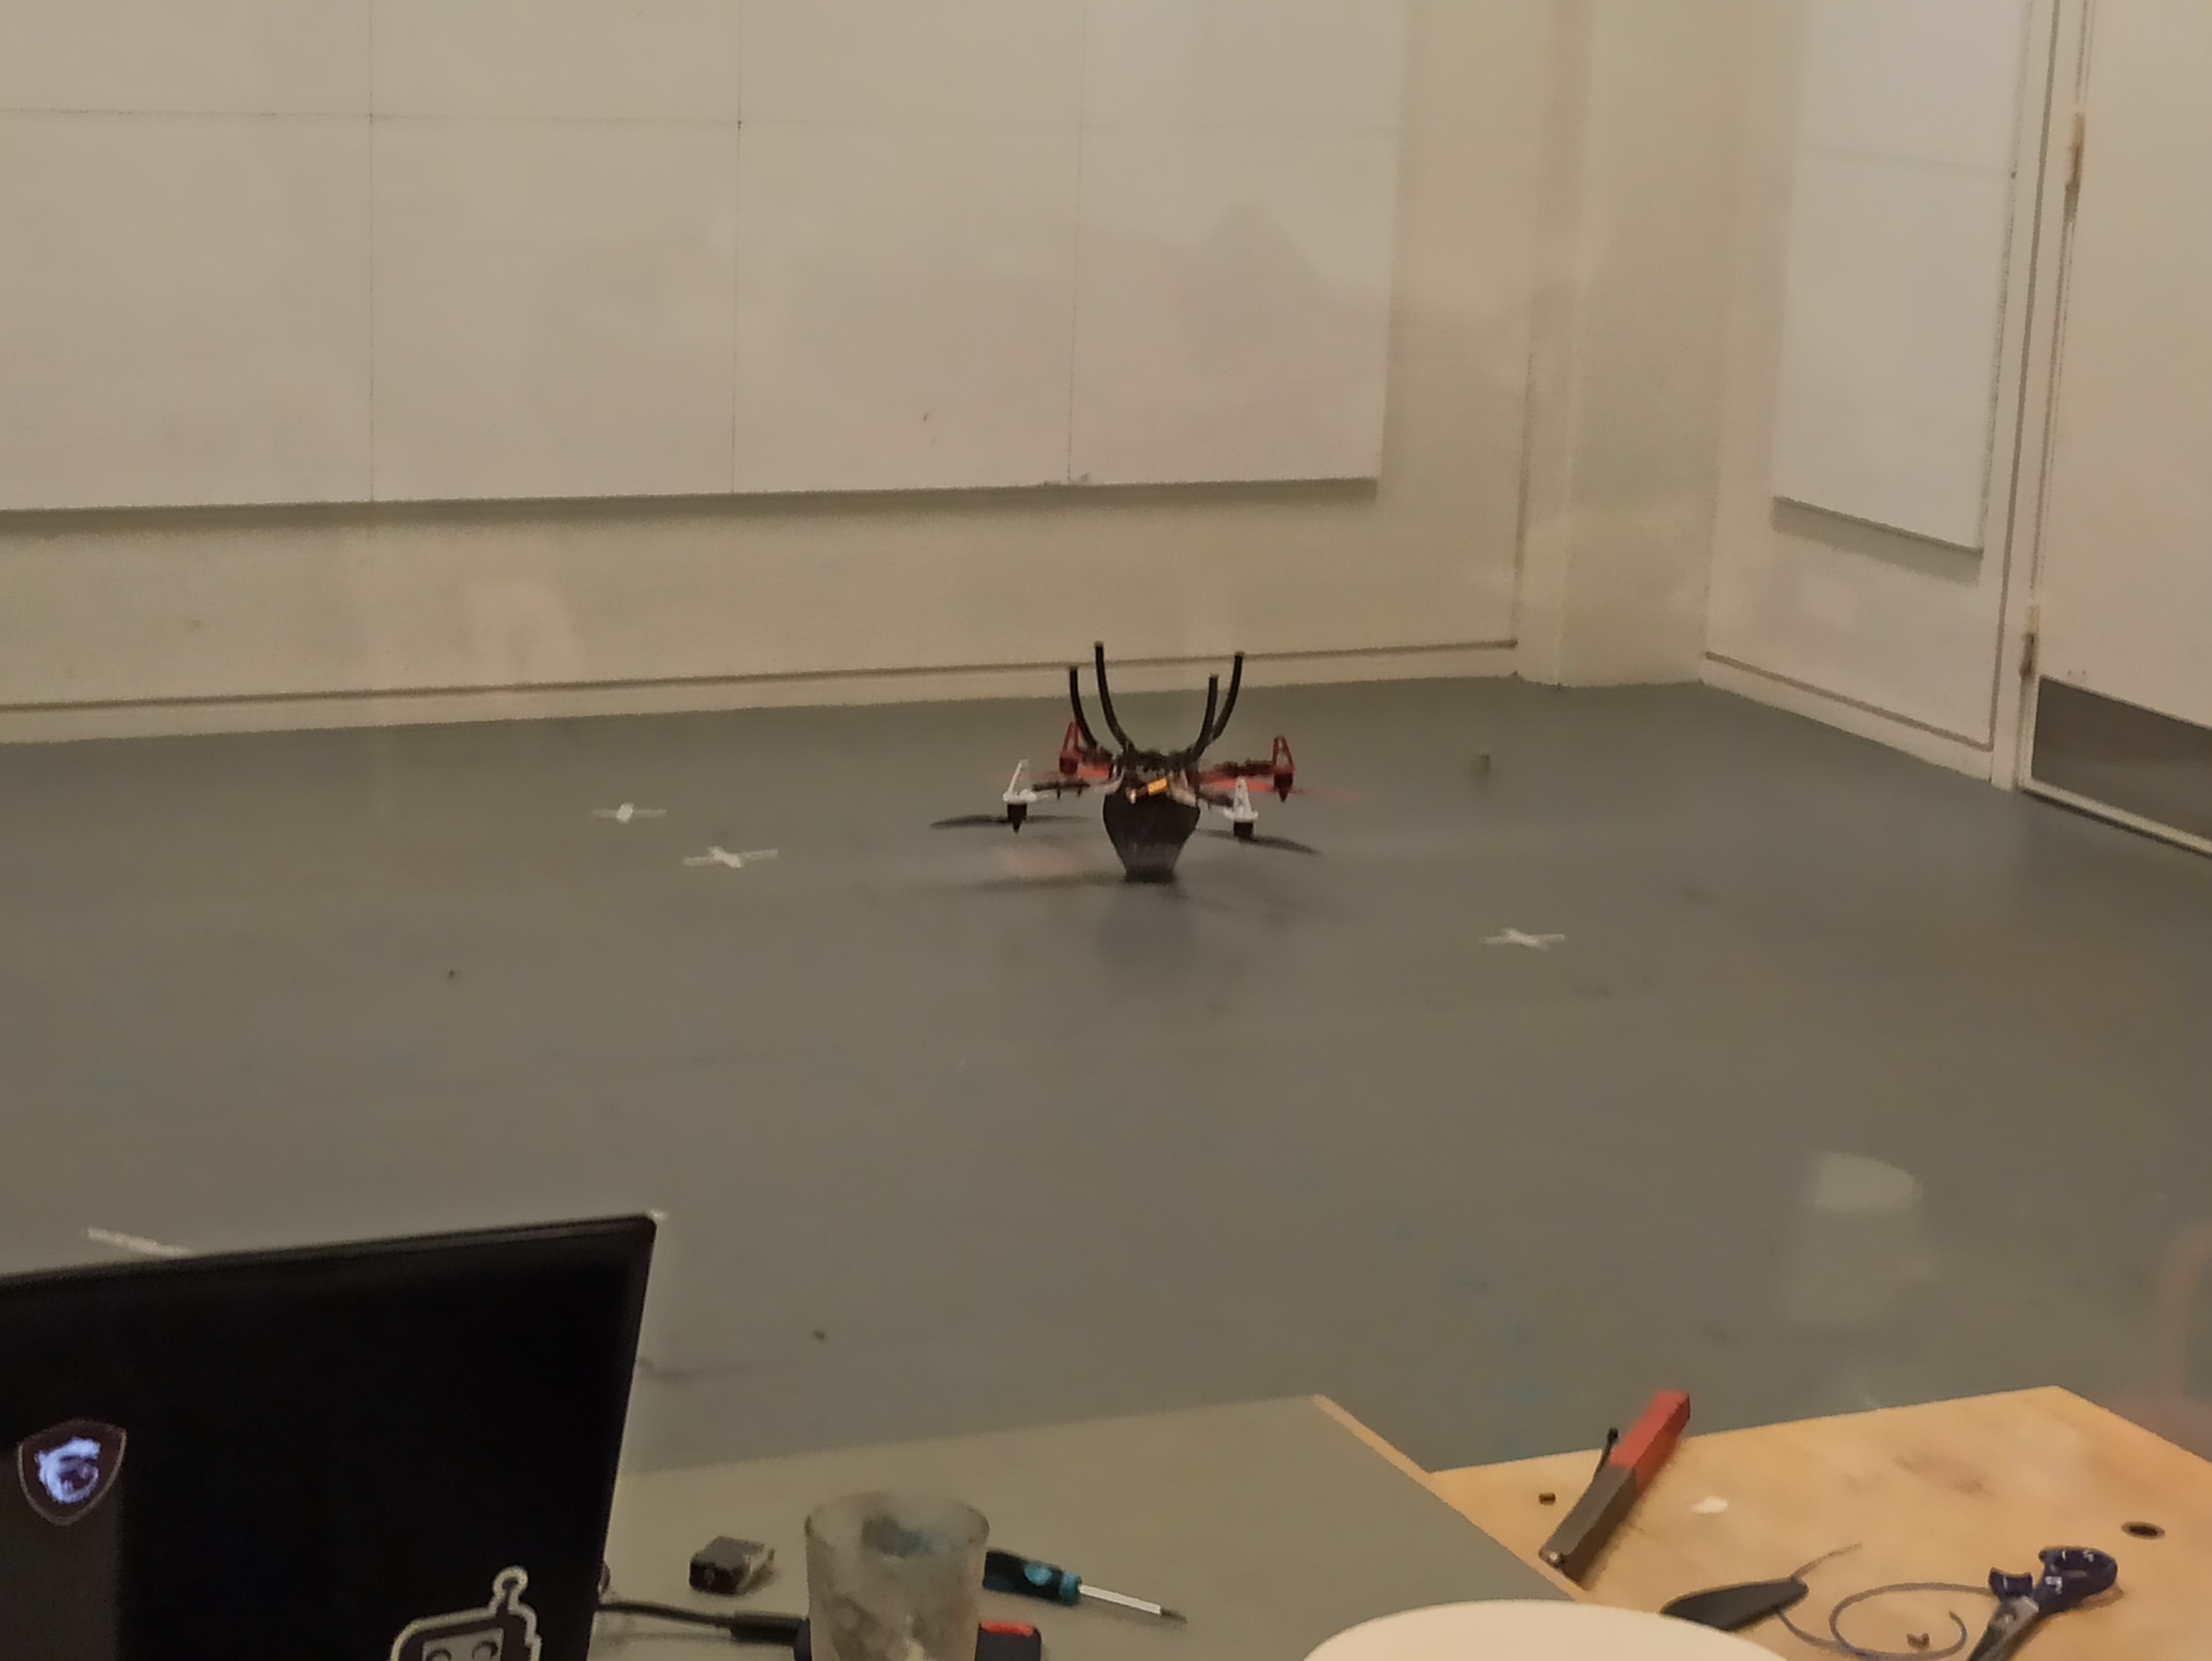
\includegraphics[width=\textwidth]{Figures/testing/SURPISEEE.jpg}
    \caption{The cover is able to protect the propellers when landing upside down.}\label{fig:test_lmao}
\end{figure}
\chapter{Conclusion}\label{ch:concl}
Four drones were developed with all the hardware specifications  required for an autonomous drone as mentioned in the Chapter \ref{ch:hw}, which is the first objective of the project \ref{sec:prob_analysis}. 

A working flight controller was also successfully developed with all the sensors capabilities (with individual test files) in Patmos multi core architecture, which is the second objective of the project \ref{sec:prob_analysis}. 

The drone manual control functionalities were tested as shown in Chapter \ref{ch:test}. The drone can be manually controlled to takeoff, fly. But the landing is not smooth because the gains have to  be fine tuned as mentioned in Subsec. \ref{subsec:altitude_hold}. Hence third objective \ref{sec:prob_analysis} is only partially fulfilled.

The altitude hold and position hold functionalities could not be implemented due to the time constraints and issues faced when working on core 3 of the multi core architecture as mentioned in Subsec.  \ref{subsec:altitude_hold}, \ref{subsec:position_hold} This is because, 
\begin{itemize}
    \item GPS and telemetry which could not tested together with flight controller due to issues in core 3. 
    \item PID values not tuned for barometer altitude control.
\end{itemize}
Due to these reasons, the final developed drone is run on multi core architecture with only manual control capability using an IMU. Thus fourth objective \ref{sec:prob_analysis} is not fulfilled.


The core 3 of the Patmos architecture, is assigned to send and receive UART data according to the flight controller designed. The data sharing between multiple cores is possible by locking the cores and updating the global variable throughout all cores. But when working on UART data, locking and unlocking cores hangs the entire program.

To explain the reason for issues on core 3, it is necessary to explain briefly how the cores are programmed inside Patmos: the user must  program the handling of access to hardware and low-level resources between the cores. Thus the issue regarding core 3 might be due to, different cores calling to functions that lock and unlock these resources without a predefined schedule or priority.

 This might be also be, due to the fact that the UART data needs to lock the access to a shared library, so it can manipulate using strings and other functions that are relatively slow. This library has also another essential resources for the other cores and therefore, the program loop speed is compromised when the GPS and telemetry are added to the flight controller. 

The developed quad-rotor design is built in a modular way with most of the components being easily replaceable. This facilitated to build multiple drones at the end of this project. Thus the fifth objective \ref{sec:prob_analysis} is fulfilled.

Apart from that, the drone simulation could not be completed, as explained in Section \ref{sec:simulation}, which could have sped up the PID tuning process. However, the communication between the simulator and the board was successful, so the simulation model could be further improved in the future.

This project has an immense scope for improvement, due to all the sensor packages developed for the FPGA. Using the existing resource and extra time, this project can be finished by implementing the remaining functionalities and can also be extended to a full autonomous implementation.



\vfill % <- use this to avoid big blank spaces
% ================================ Others ===========================


\bibliography{bibliography.bib}

\chapter{Appendix: how to assemble the drone}\label{app:build}
This chapter describes how to build and assemble all the components for both drone models presented in Chapter \ref{ch:hw} and it is useful for readers that do not find the present hardware design intuitive or that are not familiar with these DIY projects.

\section*{Board and sensors}

\begin{enumerate}
    \item On the PCB bottom side, soldier sets of female pins for the ADC module and the GPIO0. 
    On the top side, soldier the resistances and sets of male pins for the ESCs, telemetry and GPS-compass; soldier sets of female pins for the receiver, UART-USB adapter, the barometer and IMU.
    
    
    For the battery feedback and power supply pins (for the FPGA, and the +5v coming from the power module in Model-B units) the ground pins are male and voltage input are female.
    
\begin{figure} [H]
    \centering
    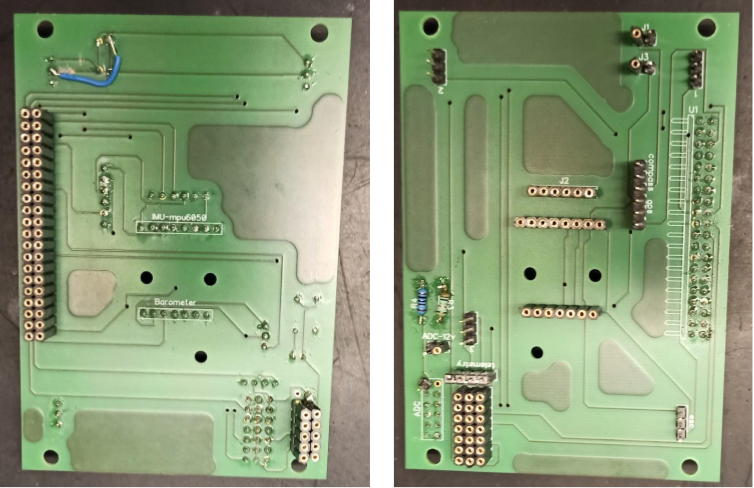
\includegraphics[scale=0.5]{Figures/build/PCB_topBottom.png}
    \caption{Pins soldier to the PCB on the bottom side (left) and top (right).}
    \label{fig:build_pins}
\end{figure}
    
    \item To attach the PCB to the FPGA, it is necessary to make the female pins on the bottom side longer, so add a second round of female pins on top of the soldiered ones. Once the PCB can be placed on top of the FPGA, use screws M3 on the corners to attach it.
    
    
    \item Add the IMU, barometer, UART-USB adapter and receiver to the top side of the PCB. Watch out for the height of the sensors.
    
    
    \item Attach the steppers to the central holes of the FPGA-Frame attachment. Afterwards, attach the part to the bottom of the FPGA.
    
\end{enumerate}


\begin{figure} [H]
    \centering
    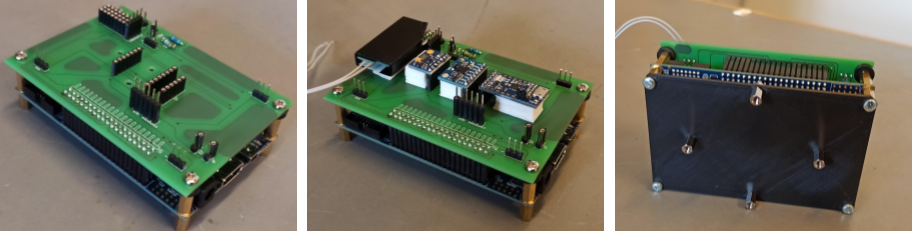
\includegraphics[width=\textwidth]{Figures/build/PCB_FPGA.png}
    \caption{Board building steps nr.2 (left), 3 (center) and 4 (right).}
    \label{fig:build_board}
\end{figure}

\section*{Main body assembly}

\begin{enumerate}
    \item Soldier the ESCs power supply and battery X66 connector to the bottom part of the frame.
    
    \item Soldier as well two additional wires for the battery feedback on the top-right ESC. It is not mandatory that the wires are blue, but this color was chosen for this project since it makes it easier to differentiate from the other components.
    
    \item Screw the arms and legs to the bottom part of the frame. Also attach with a zip or tape the ESCs to the arms. As a convenience, the two red arms are meant for the front side and the two white for the back.
    
    \item Turn the body upside down and screw the top part of the frame (except for the screws that are for the cover).
    
\begin{figure} [H]
    \centering
    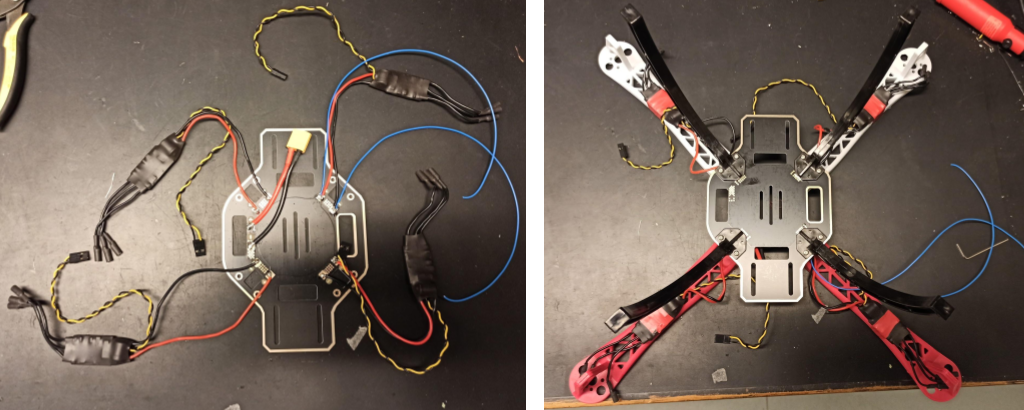
\includegraphics[width=\textwidth]{Figures/build/frame_123.png}
    \caption{Frame building steps nr.1 and 2 (left), 3 and 4 (right).}
    \label{fig:build_frame1234}
\end{figure}
    
    \item Screw the motors on the arms and connect them to the ESCs. DO NOT zip/tape these connectors yet.
    
    \item Add a belt for the battery on the bottom. In case of building a Model-B unit, also connect the power module to the battery connector of the bottom.
    
    \item Attach the telemetry module to the top. Watch out for the screws on the top and avoid covering the holes for the FPGA and cover.
    
\begin{figure} [H]
    \centering
    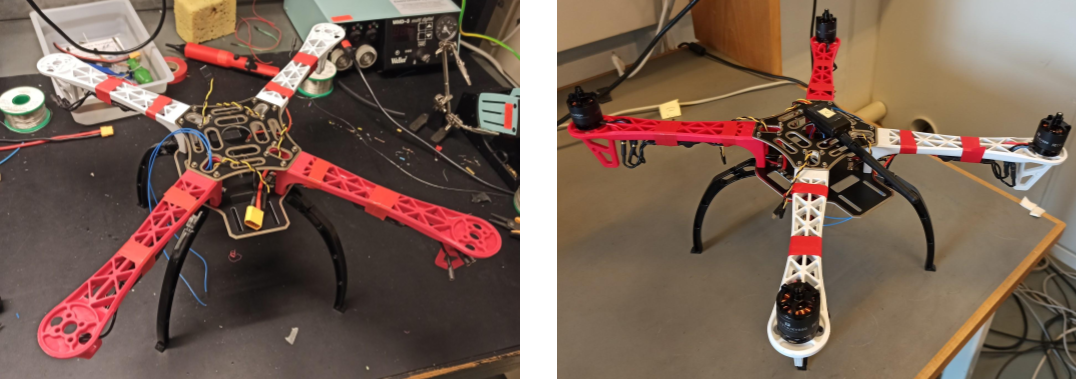
\includegraphics[width=\textwidth]{Figures/build/frame_45.png}
    \caption{Frame building steps nr.5 and 6 (left), 7 (right).}
    \label{fig:build_frame567}
\end{figure}

    \item Attach the FPGA+PCB from the previous section with the steppers. Notice that the IMU's X axis must point to the front. For a more visual understanding, the receiver placement must be between the two red arms.
    
    \item Connect the ESCs, telemetry and battery feedback to the board.
    
    \item To download a C-App without removing the cover, add a USB connector (male USB-B mini - female USB) that goes from the UART-USB adapter to the outside of the frame (just down the bottom part, see Figure \ref{fig:hw_space}).
    
    \item Add the drone number to the cover and attach the GPS to its cavity using the CGPS-Cover attachment. It is not mandatory that the drone number is the same as the telemetry pair number, but this makes it easier for working with multiple drones.
    
\begin{figure} [H]
    \centering
    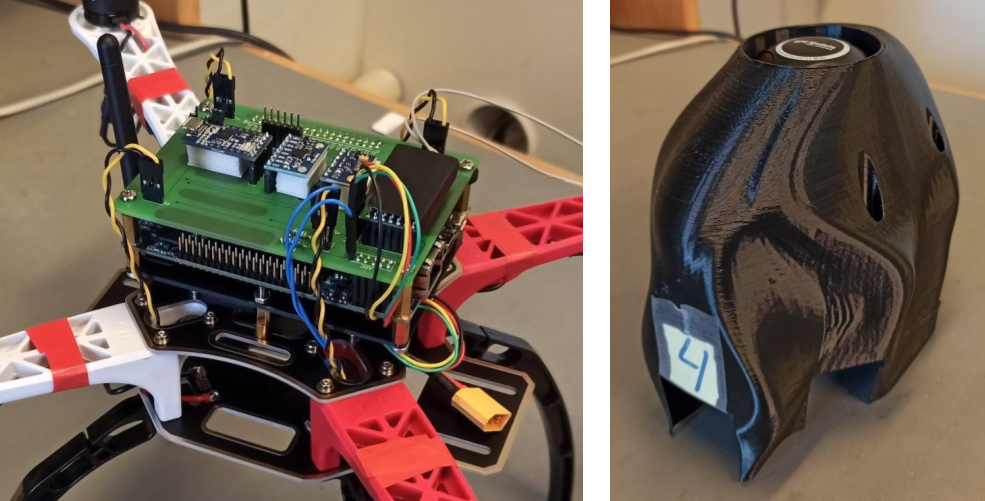
\includegraphics[width=\textwidth]{Figures/build/frame_board.png}
    \caption{Frame complete wiring (left) and finished cover (right).}
    \label{fig:build_frameBoard}
\end{figure}
    
    \item Connect the GPS to the PCB and screw the cover to the frame.
    
    \item In case of using a brand new set of motors, run the ESC calibration program to enable the motors and make them work properly.
    
    \item Run the test program for the motors and verify that the four motors spin in the correct direction. In case a motor spins in the wrong direction, switch two of its connections with the ESC.
    
\end{enumerate}

\textbf{\textit{NOTE:}} Before attaching the cover to the frame, check that the devices and the board are functional. Download Patmos and run the test programs for all the devices to verify the components are functional. Check the Appendix \ref{app:setup} to see how to do so.

In case of some devices, it is necessary to modify their settings when they are brand new (or used for the first time) in order to be compatible work with Patmos and the flight controller, see the Section \ref{app:sec_fc}.

% ===================================================================================
% Add this chapter to the table of contents:
%\addcontentsline{toc}{chapter}{Appendix: how to assemble the drone}
\chapter{Appendix: how to set up the drone}\label{app:setup}
This appendix describes how to set up the drone to take off and it is useful for readers that are not that familiar with the Patmos architecture or that want to further develop the flight controller.
Most of the following sections show parts of scripts and commands that can be found on the Patmos Handbook \cite{bib:patmos_hnd} or in the support and complementary PREDICT repository \cite{bib:pred_repo}.

For the set up, it is necessary to use computer with Ubuntu 18 at least. In case of not having one, it is possible to use the Virtual Machine (VM) provided by the Patmos main webpage \cite{bib:patmos_page}.

On top of that, this project uses the multi-core feature, which needs the external memory on the microSD of the De10-Nano board. Before downloading Patmos on the board, it is necessary to flash the SD card in order to make it compatible with the system. Files available in \cite{bib:microSD} and detailed description on the README.md in the Quartus Prime project for de10-nano-drone.

\section*{Running Patmos on the board}
The model used in this project is the FPGA De10-Nano from Altera and the Patmos OS is implemented in a Quartus Prime project. To download it on the board from a computer, it is necessary to follow two processes: install Patmos dependencies on the computer and connect it to the board.

To install Patmos:
\begin{enumerate}
	\item Create a folder called "t-crest" on your home address.
	\item Download and rename the following repositories from the T-Crest project \cite{bib:tcrest_repo}.

\lstset{style=Bstyle}
\begin{lstlisting}[language=bash]
mkdir t-crest && cd ~/t-crest
git clone https://github.com/t-crest/aegean.git
git clone https://github.com/t-crest/argo.git 
git clone https://github.com/t-crest/patmos-compiler-rt.git compiler-rt
git clone https://github.com/t-crest/patmos-gold.git gold
git clone https://github.com/t-crest/patmos-llvm.git llvm
git clone https://github.com/t-crest/patmos-misc.git misc
git clone https://github.com/t-crest/patmos-newlib.git newlib
\end{lstlisting}

	\item Delete the previous build folders.

\begin{lstlisting}[language=bash]
rm -rf ~t-crest/newlib/build
rm -rf ~t-crest/patmos/hardware/build
\end{lstlisting}

	\item Re-build and compile the libraries

\begin{lstlisting}[language=bash]
cd misc
cp build.cfg.dist build.cfg
./build.sh
cd ..
./misc/build.sh newlib
cd patmos/doc
make
\end{lstlisting}
	
	\item Check if the commands are available.
\begin{lstlisting}[language=bash]
Still on process
\end{lstlisting}

    \item In case that Patmos has been updated (new features has been added, another model has been included, etc), it is necessary to update accordingly.
    
\begin{lstlisting}[language=bash]
cd ~/t-crest/
gitall pull
# Repite build and compilation process from here
\end{lstlisting}    

\end{enumerate}

To download Patmos on a de10-nano board for the first time, it is necessary to set up some additional configuration:
\begin{enumerate}
	\item Install the FPGA drivers on the computer. The drivers must be located on the /dev/ folder, in a file. It's possible either to copy the file \textit{51-usbblaster.rules} from the complementary repository\cite{bib:pred_repo} or generate it with the following content:
	
\lstset{style=OtherSt}
\lstinputlisting{Figures/setup/Files/51-usbblaster.rules} 	

	\item Give to the computer user account the right to access the communication ports.
	
\lstset{style=Bstyle}
\begin{lstlisting}[language=bash]
sudo usermod -a -G dialout user
# Now log out from the computer and sign in again
\end{lstlisting} 

	\item Connect a FPGA to the computer and check if it can be recognised.
	
\begin{lstlisting}[language=bash]
jtagconfig
# In case the command gets stuck, kill it and re-run it
sudo killall -9 jtagd
\end{lstlisting} 	

%\end{enumerate}

\begin{figure}[H]
    \centering
        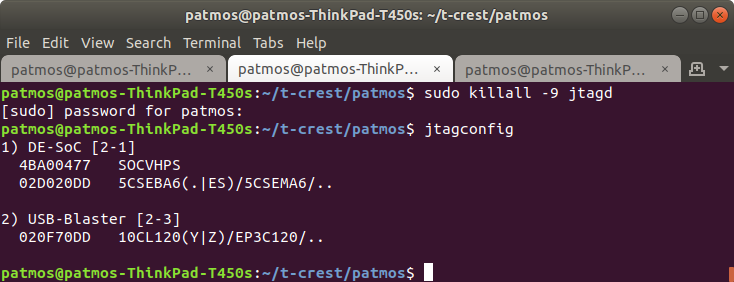
\includegraphics[scale=0.5]{Figures/setup/jtagconfig.png}
    \caption{Running the jtagconfig command shows every connected FPGA. In this case, it shows a de10-nano (De-SoC) on port 2-1 and a de2-115 (USB-Blaster) on port 2-3.}
    \label{fig:jtagconfig}
\end{figure}

Finally, to download the Quartus Prime project on the board it is necessary to compile the Patmos folders according to a certain model. Afterwards, the FPGA shall retain the architecture in its memory even after turning on and off. 
In case a C app does not run correctly, repeat only the last steps inside Quartus Prime. In case the issue still persists, repeat this procedure:
%\begin{itemize}
    \item Check that selected board is de10-nano-drone and that the communication type is DE-SoC. This is set up in the Makefile located in \textit{~/t-crest/patmos}:

\lstset{style=Bstyle}
\begin{lstlisting}[language=bash]
# Altera FPGA configuration cables
#BLASTER_TYPE=ByteBlasterMV
#BLASTER_TYPE=Arrow-USB-Blaster
BLASTER_TYPE?=DE-SoC 
#BLASTER_TYPE?=USB-Blaster

# The Quartus/ISE project
#BOARD=ml605oc
#BOARD=bemicro
#BOARD?=altde2-70
#BOARD?=altde2-115
BOARD?=altde10-NANO-oc
\end{lstlisting} 
    
    \item Check the hardware configuration for the de10-nano-drone. For this flight controller, four cores are required and the sensors are distributed and assigned between the different cores. The configuration can be checked on the \textit{~/t-crest/patmos/hardware/config/de10-nano-drone.xml}:
    
\lstset{style=Bstyle}
\begin{lstlisting}[language=bash]
<patmos default="default.xml">
  <description>Configuration for de10-nano board for drone with external ddr3 memory</description>

  <frequency Hz="50000000"/>
  <pipeline dual="false" />
  <cores count="4" />
  <ExtMem size="1g" DevTypeRef="DDR3Bridge" />

  <IOs>
  <IO DevTypeRef="Uart1" offset="6" core="3"/>
  <IO DevTypeRef="Uart2" offset="7" core="3"/>
  <IO DevTypeRef="Leds" offset="9" core="0"/>
  <IO DevTypeRef="I2CMaster" offset="11" core="1"/>
  <IO DevTypeRef="Actuators" offset="12" core="2"/>
  <IO DevTypeRef="SPIMaster" offset="14" core="0"/>
  </IOs>

  <Devs>
    <Dev DevType="Uart1" entity="Uart" iface="OcpCore">
      <params>
        <param name="baudRate" value="9600"/>
        <param name="fifoDepth" value="16"/>
      </params>
    </Dev>
    <Dev DevType="Uart2" entity="Uart" iface="OcpCore">
      <params>
        <param name="baudRate" value="115200"/>
        <param name="fifoDepth" value="128"/>
      </params>
    </Dev>
    <Dev DevType="Leds" entity="Leds" iface="OcpCore">
      <params>
        <param name="ledCount" value="8"/>
      </params>
    </Dev>
    <Dev DevType="I2CMaster" entity="I2CMaster" iface="OcpCore">
      <params>
        <param name="i2cBitRate" value="100000" />
      </params>
    </Dev>
    <Dev DevType="Actuators" entity="Actuators" iface="OcpCore">
      <params>
          <param name="extAddrWidth" value="16" />
          <param name="dataWidth" value="32" />
      </params>
    </Dev>

    <Dev DevType="SPIMaster" entity="SPIMaster" iface="OcpCore">
      <params>
          <param name="slaveCount" value="1" />
          <param name="sclk_scale" value="1" /> 
          <param name="fifoDepth" value="6"/>
          <param name="wordLength" value="12"/>
      </params>
    </Dev>

    <Dev DevType="DDR3Bridge" entity="DDR3Bridge" iface="OcpBurst" />
    <Dev DevType="OCRam" entity="OCRamCtrl" iface="OcpBurst">
      <params>
         <param name="sramAddrWidth" value="19" />
      </params>
    </Dev>
  </Devs>
</patmos>
\end{lstlisting}
    
    \item Compile Patmos for the de10-nano-drone set up. This can be done either all at once or per steps. In case of errors, it is recommended to do it per steps according to the Handbook\cite{bib:patmos_hnd} and check where the compilation fails.

\lstset{style=Bstyle}
\begin{lstlisting}[language=bash]
cd ~/t-crest/patmos
export BOARD=de10-nano-drone
rm -rf ~/t-crest/patmos/hardware/build
make gen
make -C hardware verilog BOOTAPP=bootable-bootloader BOARD=de10-nano-drone
make synth
\end{lstlisting} 
    
    \item Open Quartus Prime. The de10-nano-drone project is located in \textit{~/t-crest/patmos/} \textit{hardware} \textit{/quartus/de10-nano-drone/patmos.qpf}. In the case the project is not compiled yet, run "Compile Design" on the Task bar, to convert the project to a .sof binary file. 

\begin{figure}[H]
    \centering
        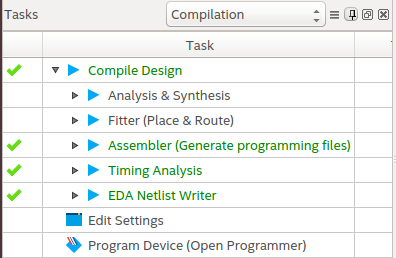
\includegraphics[scale=0.5]{Figures/setup/quatus_compile.png}
    \caption{If during the compilation in Quartus Prime errors were given, review the hardware settings, such as the board model, cores number, etc.}
\end{figure}

    \item By default, the compiled projects have the extension .sof and they are volatile, which means that after the FPGA is restarted, the Quartus project must be downloaded again. This is also an issue for using the multicore feature. To make the project permanent, it is necessary to convert the .sof into a .jic file. On Quartus Prime, go to \textit{Files/Convert Programming Files...} and generate the .jic file with the following options:
    
\begin{figure}[H]
    \centering
        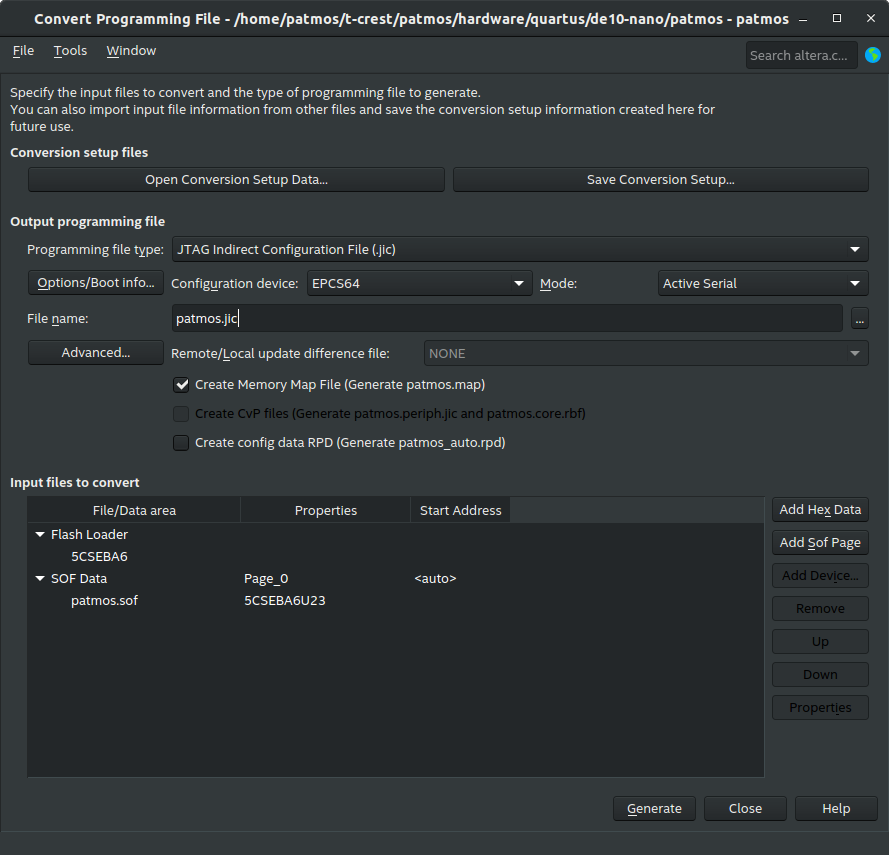
\includegraphics[width=\textwidth]{Figures/setup/quartus_create_jic.png}
    \caption{Convert Programming Files options overview.}\label{fig:app_jic}
\end{figure}    
    
    \item Open the "Program Device" (see the Figure of the Task bar) and it will open a window for downloading the project on the board. Use "Hardware Setup..." to select the DE-SoC port and "Change Files..." to select the .jic project. Notice that it is also necessary to check "Factory default enhanced SFL image".

\begin{figure}[H]
    \centering
        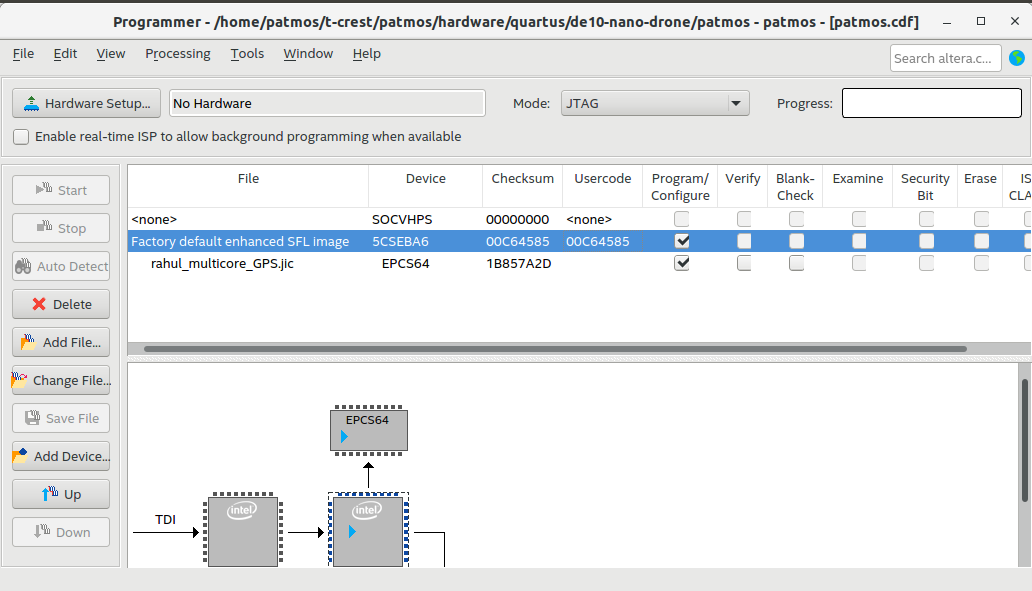
\includegraphics[width=\textwidth]{Figures/setup/quartus_download_jic.png}
    \caption{Download de10-nano-drone project window.}
\end{figure}  
    
    \item After the project is downloaded, re-start the FPGA to be able to download C-apps.

%\end{itemize}
\end{enumerate}

\section*{C apps development through a "Hello World!" tutorial}

This tutorial explains how to create a "Hello World!" C application from scratch and run it on a board.
Before starting, it is necessary to have built and downloaded Patmos as mentioned in the previous sections.  

\begin{enumerate}
    \item Create a folder for the application inside Patmos' app directory. The directory must have the same name as the app.
\lstset{style=Bstyle}
\begin{lstlisting}[language=bash]
cd ~/t-crest/patmos/c/apps && mkdir hello   
\end{lstlisting} 
    \item Create a hello.c file inside the folder with the following content:
\lstset{style=Cstyle}
\begin{lstlisting}
#include <stdio.h>
#include <machine/patmos.h>
#include <machine/spm.h>

int main() {
  printf("Hello wrold!\n");
  return 0;
}      
\end{lstlisting} 
    \item Create a Make file inside the folder, which shall compile the .c file. The \textit{patmos-clang} command transforms the .c main file (and its dependencies) into a binary file compatible with the FPGA. This Makefile contains the following:
\lstset{style=OtherSt}
\lstinputlisting{Figures/setup/Files/Makefile}    
    \item Copy the generated file to the temp directory. This can be done as well inside the Makefile (uncomment last line).
    \item Go back to the main Patmos directory and download the app.
\lstset{style=Bstyle}
\begin{lstlisting}[language=bash]
cd ~/t-crest/patmos/
make APP=hello download
\end{lstlisting} 

\end{enumerate}

\begin{figure}[H]
    \centering
        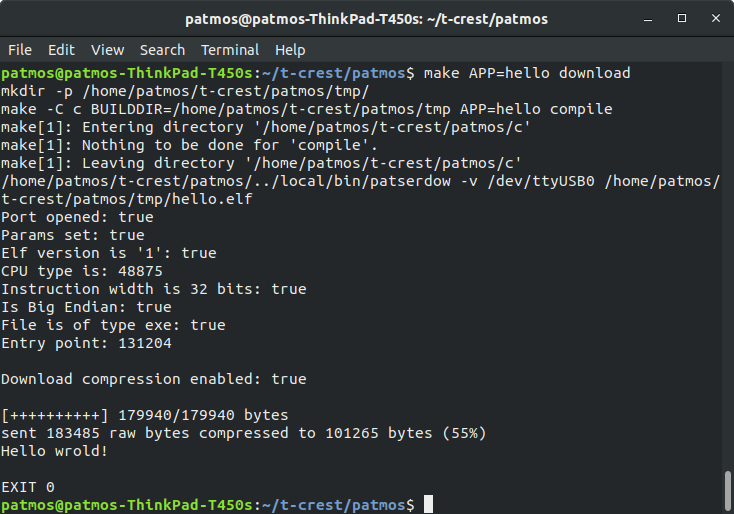
\includegraphics[scale=0.5]{Figures/setup/hello_example.png}
    \caption{Log and result on the terminal after downloading a C app.}
    \label{fig:c_app}
\end{figure}

\section*{Using the Flight Controller}\label{app:sec_fc}

The C-Application for the flight controller and its dependencies are in the \textit{~/t-crest/patmos/} \textit{c/apps/de10-nano/} directory. It contains the main script \textit{Flight\_controller\_2.c} in and the functions for each core are in the header \textit{PREDICTthread.h}. Apart from that, it also contains the following directories:

\begin{itemize}
    \item basic\_lib: contains low-level functions to access the pins and other Patmos-related options (such as counting time, etc). It also contains global variables to access the components and save their outputs, and the additional dependencies for using the GPS and barometer.
    \item FC\_functionalities: contains specific features for flying, such as the PID controller, take off, landing and calibration process.
    \item sensors: contains the handlers and implements the full functionalities for each sensor. These headers use the low-level functions from the basic library to access the sensors data and process it.
    \item sensors\_test: contains a set of different scripts. Each script is meant to be used of a specific single sensor or type of devices.
\end{itemize}
\subsubsection*{Pairing Transmitter and Receiver}\label{trans_receiver_pair}
To pair a transmitter and a receiver:
\begin{enumerate}
    \item Add the binding plug shorting the ground and the signal pins on the receiver.
    \item Power on the receiver and the receiver binding mode is indicated by fast blinking.
    \item Push the bind button on the transmitter and switch it on.
    \item The receiver is bound successfully if it stops blinking.
    \item Now remove the binding plug and the receiver is now paired.
\end{enumerate}

\subsubsection*{Change baud rate of Telemetry}\label{telemetry_baud}
The telemetry modules have to configured to be in the baud rate 115200 using a the software used by the telemetry module \cite{bib:ardupilot} (differs based on the provider of the module). 


\subsubsection*{Tuning the PID gains}
In case the behaviour of the flight controller needs to be tuned, the variables storing the PID gains can be found in the \textit{FC\_global.h} file in the \textit{basic\_lib} folder.

The recommended tuning procedure is described in Section \ref{app:tuning}.

\subsubsection*{Downloading the code}


To download this application on a board:

\begin{itemize}
    \item Select on the Makefile the main script (either the flight controller or one of the test programs available). All the dependencies have been included in this Makefile, do not change something else unless it is necessary.
    
    \lstset{style=Bstyle}
    \begin{lstlisting}[language=bash]
# Uncomment this for using the flight controller
MAIN?=Flight_controller_v2

# Uncomment and/or modify this for running a test program
# MAIN?=sensors_tests/receiver_test

# Modify this if another port is in used
SERIAL?=/dev/ttyUSB0

# Do not modify any further
I2C?=basic_lib/i2c_master
GPS?=basic_lib/gps
LDFLAGS?= \
        -mpatmos-method-cache-size=0x1000 \
        -mpatmos-stack-base=0x080000 -mpatmos-shadow-stack-base=0x078000 \
        -Xgold --defsym -Xgold __heap_end=0x070000

all:
	patmos-clang -I ../.. -O2 $(LDFLAGS) $(I2C).c $(GPS).c $(MAIN).c -o de10-nano.elf -lm
	patmos-clang -I ../.. -O2 $(LDFLAGS) $(I2C).c $(GPS).c $(MAIN).c -o ~/t-crest/patmos/tmp/de10-nano.elf -lm
download:
	patserdow -v $(SERIAL) de10-nano.elf
    \end{lstlisting} 
    
    
    \item Compile the App and download it.
    
\lstset{style=Bstyle}
\begin{lstlisting}[language=bash]
cd ~/t-crest/patmos/c/apps/de10-nano
make
cd ../../..
make APP=de10-nano download
\end{lstlisting} 

\end{itemize} 


\section*{Common troubleshooting}

\begin{itemize}
    \item Sensors and actuators: the different components can be tested individually with their own test programs. In case a specific device seems not to work properly, there are some approaches that you can try:
    \begin{itemize}
        \item In case of using the PCB for attaching the device, review the pins connection with a voltimeter. Follow the hardware diagram and connections shown in Chapter \ref{ch:hw}.
        
        \item In case of not using the PCB and connecting the device directly to the board, review the wiring and power supply. Sometimes it can be that two connections are accidentally switched (TX and RX, or SCL and SDA).
        
        \item Check that the device is not faulty and properly on. In a nutshell: IMU must light green, the barometer GPS+compass light red, the telemetry lights permanently green and the receiver red.
        
        In case the telemetry module is blinking green, it means it cannot reach its paired module, so it is necessary to review the connection between modules.If it permanently red is on configuration status, which means it needs to be connected to a computer with SikRadio \cite{bib:ardupilot} and its firmware needs to be re-uploaded. 
        
        In case the receiver is blinking-slow red, it means it cannot reach its paired transmitter, so review that the transmitter is properly on and paired to it. In case the receiver is blinking-fast red, it is on pairing mode and it needs to be paired with a transmitter and restarted afterwards, see Section \ref{app:sec_fc}.
        
        \item In case the device seems to be working fine, it could be that it is assigned to the wrong core or with the wrong settings. Review the hardware settings on the \textit{de10-nano-drone.xml}.
        
        Then modify Patmos configuration to single-core and with all the devices assigned to core 0. Then change the test program to one single thread with the function for that specific device.
    \end{itemize}
    
    \item Compiling Patmos: a server compiles and builds Patmos periodically to verify it is properly set, so it should not be a problem to build it and compile in a laptop.
    
    In case of compiling Patmos when it has been updated after some time, update not just the patmos repository, but all the repositories from the t-crest folder. Then follow the presented instructions for downloading Patmos on the board. Most of the building issues come from Step 4, where the libraries are built, so try to run the $./build.sh$ from another directory or rebuilding the newlib by steps.
    
    Also review that the board model is correctly specified as $de10-nano-drone$.
    
    \item Downloading Patmos: for this specific the project, the Patmos architecture is multicore, so review first the microSD card is correctly flashed and inserted. For this project the microSD cards were flashed in a Windows computer using Windiskimager32.
    
    Review afterwards the settings for the .jic file in Figure \ref{fig:app_jic} and remember to re-start the FPGA.
    
    \item Compiling C apps: use the Patmos dependencies libraries as presented in this project and other Patmos-app examples. 
    
    Also before downloading an app, review that the generated .elf files from the C code are updated. There is a difference between compiling an App from its own folder (it generates an .elf file there) than from Patmos main directory (it generates an .elf file on the $~/t-crest/patmos/tmp$ directory), so it can be that an App is built differently depending on the process and it can also be that the .elf file downloaded on the board is outdated. 
    
    For this project, the flight controller application was built on its own folder and the Makefile would create the two .elf files.
    
    
    \item Downloading C apps: here are some of the most common issues:
\lstset{style=Bstyle}
\begin{lstlisting}[language=bash]
java.util.concurrent.TimeoutException: Receiver did not reply (715 responses missing)
jssc.SerialPortException: Port name - /dev/ttyUSB0; Method name - openPort(); Exception type - Permission denied.
\end{lstlisting} 

Review that the user account has root privileges on the ports communication, on the steps 1 and 2 from downloading Patmos.
    
\lstset{style=Bstyle}
\begin{lstlisting}[language=bash]
java.util.concurrent.TimeoutException: Receiver did not reply (715 responses missing)
jssc.SerialPortException: Port name - /dev/ttyUSB0; Method name - closePort(); Exception type - Port not opened.
\end{lstlisting} 

Review that the FPGA drivers are properly installed and that not other process has not already access the port. Sometimes the easiest way is to disconnect the FPGA, re-start it and connect it again.

\lstset{style=Bstyle}
\begin{lstlisting}[language=bash]
java.util.concurrent.TimeoutException: Receiver did not reply (715 responses missing)
jssc.SerialPortException: Port name - /dev/ttyUSB0; Method name - openPort(); Exception type - Port not found.
\end{lstlisting} 

Review that UART-USB port is properly powered up (the drone should have the battery connected) and the port number matches what it is specified on the Makefile from $~/t-crest/patmos$.
    
\end{itemize}
% ===================================================================================
% Add this chapter to the table of contents:
%\addcontentsline{toc}{chapter}{Appendix: how to set up the drone}


\end{document}